\documentclass[12pt]{extarticle}

\usepackage{amsmath, amsthm, amsfonts, enumitem, graphicx, subcaption, cleveref, tabularx, xpatch, imakeidx, setspace, mathptmx, titlesec, fancyhdr, etoolbox, tocloft, float, lipsum, amssymb, algorithm, algpseudocode}
\usepackage[font=small, singlelinecheck=off]{caption}
\usepackage[backend=biber,style=numeric]{biblatex}
\usepackage[a4paper,top=3cm,bottom=2.5cm,left=2.5cm,right=2.5cm]{geometry}
\makeindex

\addbibresource{src/bib/references.bib}

% TIPOGRAPHY
% Page settings
\pagestyle{fancy}
\fancyhf{}
\fancyfoot[C]{\thepage}

% Line spacing
\onehalfspacing

% Paragraph indent
\setlength{\parindent}{0.7cm}

% Chapter and section titles
\titleformat{\chapter}[display]{\bfseries\Huge}{\chaptername\ \thechapter}{20pt}{\bfseries\LARGE}
\titleformat{\section}{\normalfont\Large\itshape}{\thesection}{1em}{}

% Blockquote setup
\newenvironment{blockquote}{\begin{quote}\onehalfspacing\fontsize{11}{13.2}\selectfont}{\end{quote}}

% Footnotes
\renewcommand{\footnotesize}{\fontsize{10}{12}\selectfont}
\setlength{\footnotesep}{\baselineskip}
\appto\footnotesize{\singlespacing}

% CUSTOM COMMANDS
\newcommand{\meqref}[1]{Eq.\ref{#1}}
\newcommand{\mfigref}[1]{Fig.\ref{#1}}
\newcommand{\mtabref}[1]{Tab.\ref{#1}}
\newcommand{\mappendixref}[1]{Appendix \ref{#1}}
\newcommand{\indfunc}[1]{\textit{\textbf{1}}_{#1}}
\newcommand{\midcaption}[1]{
    \captionsetup{justification=centering}
    \caption{#1}
}
\makeatletter
\xpatchbibmacro{textcite}{%
  \printnames{labelname}%
}{%
  \printfield[citetitle]{labelname}%
}{}{}
\DeclareCiteCommand{\fancycite}
  {\usebibmacro{prenote}}
  {\textit{\printnames{labelname}%
   \ifnum\value{citecount}=1 \printtext{ et al.} \fi%
   (\printfield{year}) \textsuperscript{\printfield{labelnumber}}}}
  {\multicitedelim}
  {\usebibmacro{postnote}}
\makeatother
\makeatletter
%\DeclareFieldFormat{labelnumber}{\textit{\mkbibsuperscript{#1}}}
\DeclareCiteCommand{\ucite}
  {\usebibmacro{prenote}}
  {\textsuperscript{\textit{\printfield{labelnumber}}}}
  {\multicitedelim}
  {\usebibmacro{postnote}}
\makeatother

\begin{document}

\title{Properties and Implementation of Sequential Expansion of Latin Hypercube Sampling for Simulation Design}
\author{Crespi Alessandro, Gerosa Davide, Boschini Matteo}
\date{July, 2024}
\maketitle

\tableofcontents
\pagebreak

\begin{abstract}
Lorem ipsum dolor sit amet, consectetur adipiscing elit. Proin luctus finibus euismod. Quisque purus mauris, mollis sed tellus quis, congue hendrerit eros. Aliquam tempus suscipit risus non viverra. Ut pharetra mollis ante, sit amet vestibulum augue laoreet eget. Nunc tincidunt ex sit amet rutrum euismod. Maecenas feugiat, mi aliquam semper rutrum, purus justo imperdiet massa, sed feugiat leo libero sit amet sapien. Mauris sit amet sem rhoncus, hendrerit nunc sed, sagittis felis. 
\end{abstract}


\section{Introduction}
Simulation design is a branch of Statistics focused on building better simulations to enhance the comprehension of phenomena. These simulations are widely used in mathematics, physics, economics, mechanics, and other scientific fields as tools for proving theories, interpolating real sampled values, and generating predictive models to explore uncharted traits and features, perhaps intuitively or roundly developed in the early stages of the study of a specific problem.

Since the advent of hybrid mechanical-electrical programmable calculators such as IBM's machines, the first of their kind to be really useful in engineering, scientists have used them to perform heavy computations for experiments. In 1969, Kennar and Stone's Computer Aided Design for Experiments (CADEX)\ucite{kennard1969} proposal for computer-driven experiments led to spread up a broad variety of Computer-based simulation methods.

Eventually, computer-based simulations are a set of strategies that benefit from mathematical modeling techniques based on discrete known points placed in a limited parameter space, hereafter samples, and the computer programmability advantage has been used to design, shape and enhance a specific subset of samples that satisfy the desired properties, hereafter sample sets. 

The general concept of computer simulation has been defined in the past few decades, it's based on the following key ideas: taking into account a desired behavior $ F $ the experimenters have an interest in, F has to be explored through its $ N $ real parameter space; the algorithm takes samples from a standard $ N $-dimensional hyperspace $ \Omega $ and arranges the sample set for the simulation; afterwar, the simulation is carried out by evaluating $ F $ over the sample set and eventually producing a so-called surrogate model. The class of algorithms meant to implement this abstraction is commonly labeled with \textit{sampling methods}.

To the category of sampling methods belongs also the fixed-step (or determined-step) samplers, which adopt a $h(x)$ function that space samples across the hyperspace evenly or deterministically. For instance, consider $h(x)$ constant function or a Chebyshev nodes \ucite{stewart1996}. For the matter of this paper, we have focused on the sampling methods whose points are drawn with a specific random distribution.

A critical consideration when evaluating sampling methods is the trade-off between exploration and exploitation. An exploration-oriented sample set maximizes the simulation expertise of seeking key features over the studied behavior. Exploration has been depicted as a model-free practice, so that it does not base its own actions on the model (behavior) evolution or any other on-site response. On the other hand, exploitation is an auxiliary mechanism that aims to better assist the simulation by deploying samples in strategic placements that prevent exploration from exceeding the prediction surrogate made upon a key region (such as overshooting an optima or mismatching a discontinuity for a steep slope).

The most iconic sampling method for simulations is the pseudo-random sampling, lightened of every other criteria, namely the Monte Carlo Sampling or MCS (\fancycite{metropolis1987})  which has been proposed as the fundamental design of sampling methods. Quasi-Monte Carlo methods are a class of sampling algorithms based on Monte Carlo, indeed, but without a proper random drawing of sample points from the parameter space, instead, points are sequentially extracted in order to satisfy one or multiple criteria as best as the computational time required remains acceptable. Many criteria have been theorized and tested; each of them has a proper application context. An updated, summarized list of the most remarkable ones is shown and commented in \cref{tab:remarkable_criterions}. 

In the scope of this matter, the authors will focus on the space-filling class of criteria and, particularly, on the one-projection property (also known as non-collapsing property or projective property); The former measures the quality of a sample set to be spread evenly across an hyperspace; the way space-filling is defined determines the final aspect of the sampling. On the same hand, a sample set, in $P$-dimensional space, admits the one-projection property if and only if the projections of the samples on a specific dimension fall into distinct intervals $I_i$. These $I_i$ intervals are fixed-width slices of the limited volume of parameter space taken into examination (e.g., an hyper-volume $[0,1)^N$) and the number of intervals is equal to the number of samples. So, the non-collapsing property prevents samples to fall into a busy area (which has been occupied by another sample). Furthermore, given that the number of intervals and the size of the sample set is equal, it does ensure there are no empty intervals across the parameter space. This property is widely known because it is the fundamental property which Latin Hypercube Sampling sets (LHS) are based on, topic of this paper.

The authors used to work with sampling methods for simulation design, more likely LHS designs, in Astrophysics related experiments, such as simulating black hole binary mergers, which obviously requires a massive amount of computational time and many different parameters. The authors often experienced difficulties predicting how long it would take to run a full simulation given $N$ known sampling points in a $P$-dimensional space. This situation forces them to reserve more machine time on a shared company supercomputer for experiments than they really need. In order to better spend the reserved machine time left after the execution of the first run of sampling points, the authors designed an algorithm that adds up points to the initial LHS sample set using another one that has been drawn by the expansion algorithm in order to preserve the non-collapsing property of both sample sets together.\\
Differently, they have experienced another issue related to the accuracy of the surrogate model, result of the simulation consumed after the LHS set. Sometimes, it just happens that the model doesn't satisfy an eventual accuracy threshold. Instead of throwing the simulation away and compute another one, they would like to expand the current initial set with additional points to help, the updated model, converging.

The authors of this paper propose a algorithm called \textit{Expansion of an LHS} that, indeed, takes a already existing Latin Hypercube Sampling' sample set and propose a new set of points samples in the same parameter hyperspace which are suppose to maintain properties stability altogether.
The original sample set is referred as \textit{starting set} and the add-on samples as \textit{expansion set}. The whole sample set joined together by both is called \textit{expanded set}.

The paper is structured as follows: \cref{sec:lhs} yields a Latin Hypercube Sampling brief history and formal definition; in \cref{sec:lhs_expansion} is shown the research results and discussion of the expansion task issued; \cref{sec:experiments} contains metrics and experimental evaluations on the applied expansion algorithm; \cref{sec:conclusions} [...].

\section{Latin Hypercube Sampling}
\label{sec:lhs}
\subsection{What is an LHS?}
\label{subsec:what_is_an_lhs}
According to the Handbook of Combinatorial Designs \ucite{colbourn2006}, the first appearance in history of the "Latin Square" has to be attributed to the Korean mathematician Choi Seok-jeong, who described it, using modern terminologies, as a $N \times N$ matrix with $N$ distinct symbols, appearing $N$ times each but precisely once per type for each row and column. The suffix "Latin" has been inspired by the efforts that Leonhard Euler has put into this topic while defining a general theory for Latin Squares \ucite{wiki_latin_square} [working on replacing wikipedia] and using Latin letters as symbols to fill the square up with. See Fig.1 for an example with 4 objects.

\begin{figure}[h]
    \centering
    \begin{subfigure}[b]{0.45\textwidth}
        \centering
        \vtop{
        	\vspace{0pt}
        	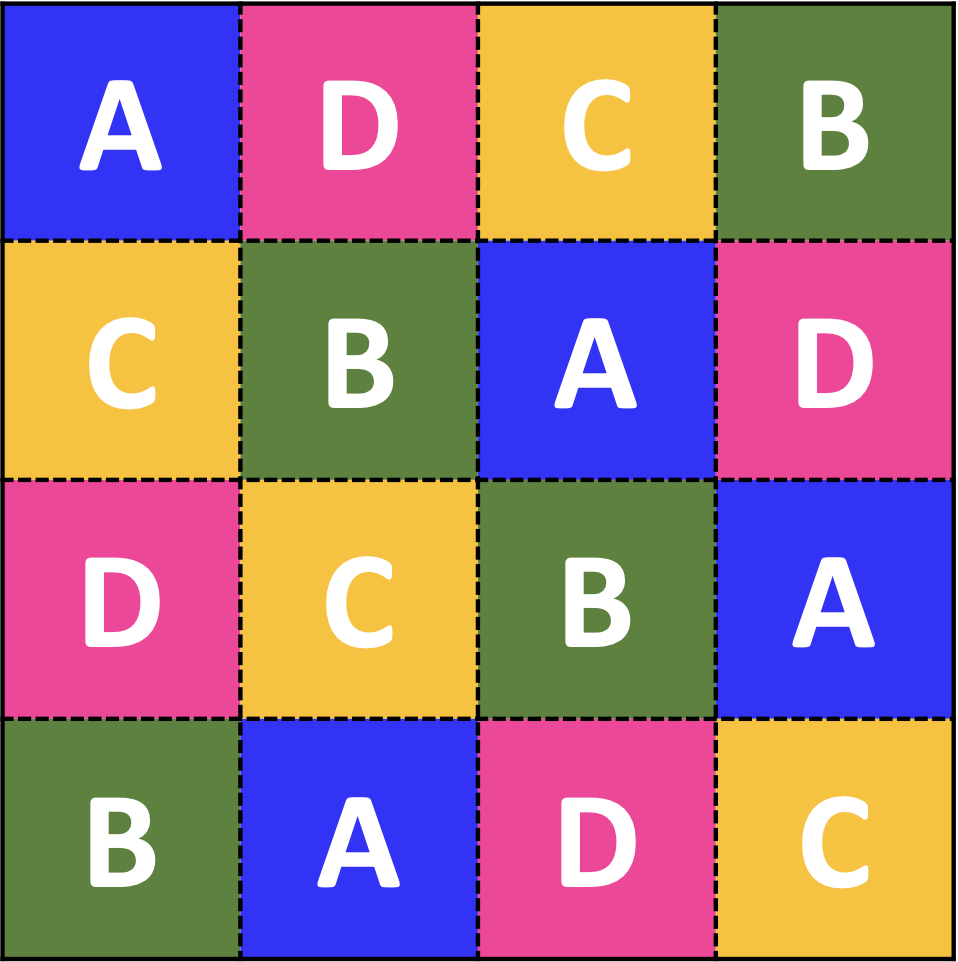
\includegraphics[width=\textwidth]{src/imgs/latin_square_letters_and_colours.png}
        	%\captionsetup{}
        	\caption{A Latin 4x4 Square with 4 distinct symbols, both letters or colors either, arranged so that no letter occurs more than once in a row or a column}
        	\label{fig:latin_square_a}
        }
    \end{subfigure}
    \hspace{0.05\textwidth}
    \begin{subfigure}[b]{0.45\textwidth}
        \centering
        \vtop{
        	\vspace{0pt}
        	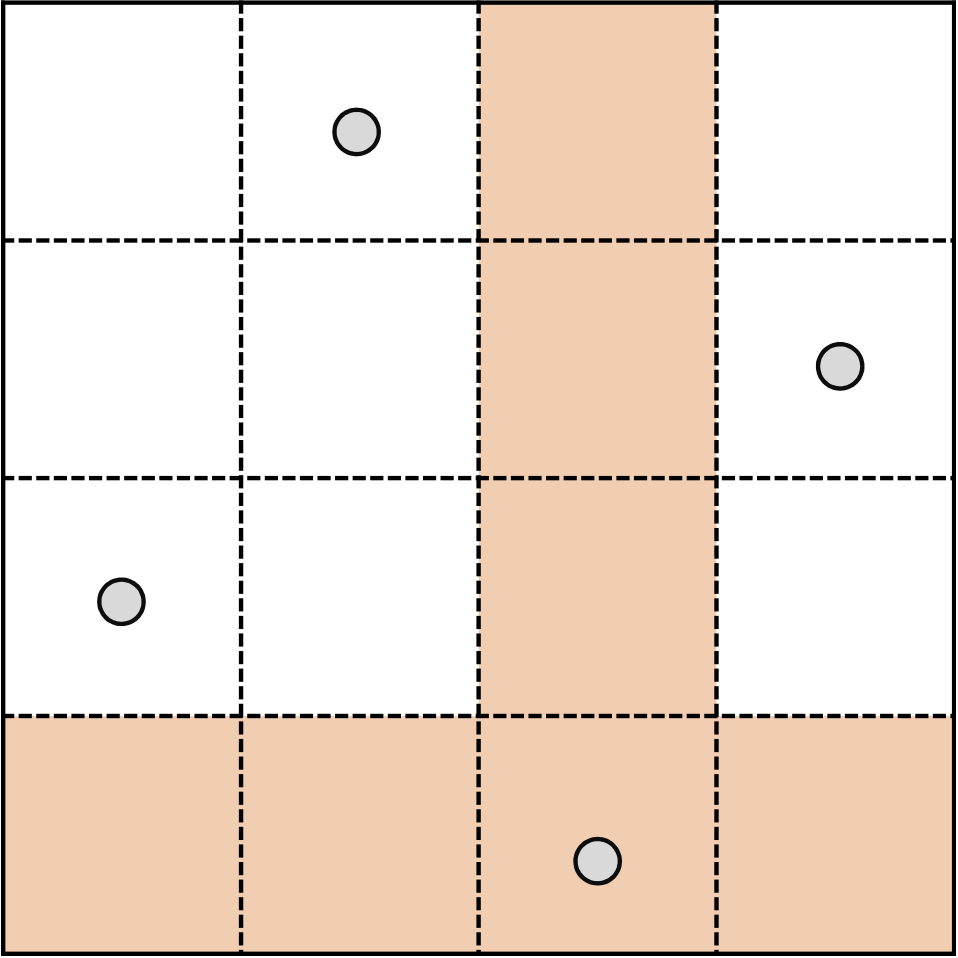
\includegraphics[width=\textwidth]{src/imgs/latin_square_skeleton.png}
        	\caption{The skeleton of (a) Latin Square highlighting only the D (or PINK) symbol positions, it's easily noticeable how the positions does not overlap onto each other's row and column both}
        	\label{fig:latin_square_b}
        }
    \end{subfigure}
    
    \midcaption{[RIFAI E NON CITARE] The images were kindly taken from \fancycite{sheikholeslami2017}}
    \label{fig:latin_square}
\end{figure}

In the scope of this paper, which doesn't aim to study combinatorial properties of $N$ symbols, we consider the placement of a sample set, which has to obey to the non-collapsing property. The symbols must occur in the matrix exactly $N$ times each. Instead of consider all symbols, we will look to a single one only. 

Generally, we can speak of modern Latin Hypercube designs as the Euler's Latin Square's matrix concept (depicted as a grid in Fig.1b) but deeming a more complex multidimensional matrix. $N$ symbols are placed in the same way of earlier, multidimensionally talking: such that each one lies exactly once on each fiber (in literature, a "fiber" of a multidimensional matrix is the general term for a one-dimensional substructure in any dimension [or mode] of a tensor. e.g. In a 2D matrix, the fibers of the first and second dimensions are respectively "rows" and "columns").
Moreover, LHS is no longer supposed to place symbols in matrices but, instead, put $N$ random samples on the hyperspace. The \textit{hyperspace} represents the examined multi-parameter space of the interested model, whereof each axis is associated with a different parameter.

By definition of LHS, the parameter hyperspace has a limited span, which is the hyper-volume $[0,1)^P$, commonly used in literature. However, some texts use a different standard, and they let the parameter space take place in a $[-1,1)^P$ hypercube. Every parameter axis is sliced into smaller consecutive intervals of width $\frac{1}{N}$ that consequently depict the sub-region where each coordinate of the points is sampled randomly. In anticipation for further definitions, we provide a indexing system for intervals; in any dimension of the hypercube with $N$ intervals, for each $i$ from 0 to $N-1$, the i-th interval's boundaries are:
\begin{equation}
\label{eq:interval_index}
I_i = \Big[\frac{i}{N}, \frac{i + 1}{N}\Big)
\end{equation}
for further usage, the right term $\frac{i + 1}{N}$ of the interval was called \textit{frontier of the i-th interval} which is shared with the left hand term of $I_{i+1}$. 
With no loss of generality, the examples and considerations designed by the authors of this paper assess the random distribution to be uniform in all intervals. The uniformly distributed samples can be transformed by associated transformation functions for any other distribution (e.g. Gaussian distribution).

\subsection{How to build a Latin Hypercube Sample Set}
\label{subsec:how_to_lhs}
In this section it has been marked out mathematically the construction of an LHS sample. This description is widely used for introducing the topic on many textbooks and lectures and it takes inspiration from the work of X.Kong at al.\ucite{kong2017}.
Let $S = \{S_1, S_2, ..., S_N\}$ be the Latin Hypercube sample set with $N$ number of samples, where $\|S_i\| = P$ number of dimensions. It is comfortable to use the matrix notation $S_{ij}$, whereof rows are the i-th sample and columns, instead, represents the projection of every sample on each j-th dimension. Then, we introduce the sorted index matrix $A = \{a_{ij} = i\}$ of $N \times P$ dimension as a tool for trace the intervals index, its purpose will be clearer soon. \\
Given an $A$ index matrix, the preliminary design matrix S is given by: 

\begin{equation}
\label{eq:Sij_def}
S_{ij} = \frac{u_{ij} + a_{ij} - 1}{N}
\end{equation}

where $u_{ij}$ is a uniform distributed variable U[0,1). This preliminary design has the peculiarity to have the samples always placed on the diagonal of the hypercube $[0,1)^P$. Now, the indexes matrix comes into use, typically shuffling the original $A$ we attain $B = \{b_{ij}\}$ random permutation, which plugging it  into \cref{eq:Sij_def} describe the uniform random variable $S_{ij}$ living inside the statistical bin identified by the interval index $b_{ij}$. We explicitly write down the uniform random variable $S_{ij}$ involving \cref{eq:interval_index} boundaries for the ij-th interval as well: 
\begin{equation}
\label{eq:rand_variable_Sij}
S_{ij} \text{ $\sim$ } U\Big[\frac{b_{ij} - 1}{N}, \frac{b_{ij}}{N}\Big)
\end{equation}

Along this paper, the authors have used the notation $R = MC(N, P)$ where MC is the Monte-Carlo sample set space of $N$ points in $P$, hence $R$ is a Monte-Carlo sample set. \\
Similarly, the expression $S \in LHS(N, P)$ states that $S$ is a Latin Hypercube sample set of the same parameters.
By definition of LHS, which stress that it is a quasi-Monte-Carlo sample set distribution, we can write that:

\begin{equation*}
LHS(N, P) \; \subset \; MC(N, P)
\end{equation*}

\subsection{Grade of a Sample Set}
\label{subsec:lhs_grade}
For the purpose of this research, the authors introduced a tool to measure how much a Monte Carlo sample set is close to a Latin Hypercube one, namely \textit{grade of a sample set}. This metric (\meqref{eq:grade}) is designed to assign to a sample set $S$ of $N$ elements in $P$ dimensions an index that ranges from the worst possible distributions of points when approaching 0 (it happens if samples overcrowd into the same very intervals and let many more empty) to a fully conventional LHS when grade equals to 1, such that:

\begin{equation}
\label{eq:grade_range}
0 < gr(S) \leq 1 \;,\; S \in MC(N,P)
\end{equation}
\\
such that
\\
\begin{equation}
\label{eq:grade_of_lhs}
gr(S) = 1 \;\Leftrightarrow \; S \in LHS(N, P)
\end{equation}
\\
The grade formula cast the arithmetical average of the presence (with numerical value 1) of the projection of every sample in each interval for each dimension:

\begin{equation}
\label{eq:grade}
gr(S) = \frac{\sum^P_{j=1}\sum^N_{q=1} min(\sum^N_{i=1}\indfunc{[\frac{q-1}{N}, \frac{q}{N})}(S_{ij}), 1)}{P \cdot N}
\end{equation}

where $\indfunc{}$ is the indicator function (see \mappendixref{appendix:indicator_function}), the variable $q$ is another way to represent the sorted index matrix $A = \{a_{ij} = i \}$ for a more immediate comprehension. The $min$ operator states that the presence of several samples' projections in a specific interval $q$ doesn't weight up the whole term, which would be at most 1 even if multiple samples lie in $q$. Hence, the grade formula ignores the overlapping samples onto the same interval, hereafter only \textit{overlaps}.

\subsection{Additional properties (Work in progress)}
\label{subsec:lhs_properties}
In this section, the authors present some very important additional properties that could greatly improve the accuracy - or the quality in other terms - of the surrogate model produced by the consumed simulation.

A well known issue with LHS designs is well depicted in \mfigref{fig:diagonal_poor_design}. It's obvious that it must be considered a poor simulation design for the most of the experiments. Usually, implementations of LHS add some peculiar properties to the design. We can highlight two superclasses of properties which LHS may be joined with: model-free properties and model-based properties.


\begin{figure}[h]
    \centering
    \begin{subfigure}[b]{0.45\textwidth}
        \centering
        \vtop{
        	\vspace{0pt}
        	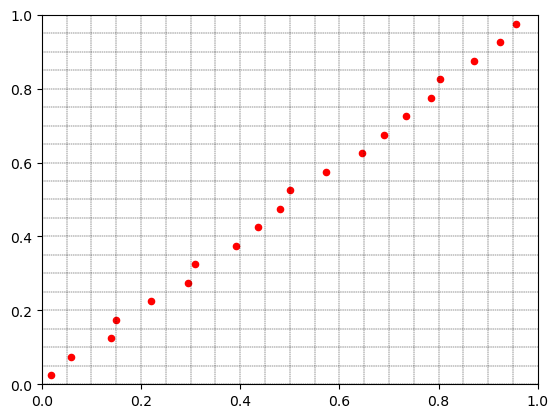
\includegraphics[width=\textwidth]{src/imgs/diagonal_poor_design.png}
        	\caption{A poor Latin Hypercube sampling in 2 dimension. Despite it fulfills the one-projection rule, it busts the experiment.\\ The diagonal sampling depicts how insufficient a pure LHS is to achieve a good simulation.}
        	\label{fig:diagonal_poor_design}
        }
    \end{subfigure}
    \hspace{0.05\textwidth}
    \begin{subfigure}[b]{0.45\textwidth}
        \centering
        \vtop{
        	\vspace{0pt}
        	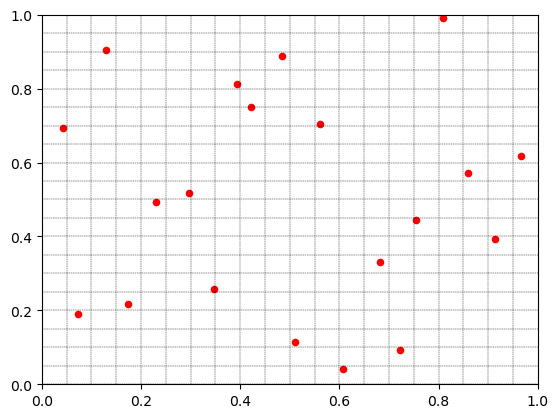
\includegraphics[width=\textwidth]{src/imgs/good_design.png}
        	\caption{LHS with space-filling property prevents samples to cluster together, low-discrepancy reduces unintentional patterns. This sampling has been generated using scipy.stats.qmc.LatinHypercube utility class. The sample generator bears random permutations of coordinates to lower the centered discrepancy \ucite{scipy_lhs}.}
        	\label{fig:good_design}
        }
    \end{subfigure}
    
	\midcaption{}
    \label{fig:latin_square}
\end{figure}

\subsubsection{Model-free and model-based simulation designs}
\label{subsubsec:model_free_model_based}
As the names may suggest, the latter implies the experimental design to involve some the peculiarities of the function to evaluate e.g. the shape that is expected, the initial or boundaries conditions, any well known critical region. Given that this approach is knowledge-driven, "What do we already know about?", can knock down pretty much the computational time required for the whole experiment with eventually high accuracy, but it can be equally easy that results may be biased, based on assumptions that may prove wrong later, or make hard any further effort from other scientists to retake the experiment and confirm the results if the assumptions are not completely clear.
On the other hand, the model-free is the formal way to depict a fully independent sampling of the parameter space from the experiment which it has been designed for. Because of not many criteria have been left, all of the properties in this class are based on inter-element relationships, which convey that for each of them has a heuristic meant to quantify how much each sample is well-placed among the others. The shorthand for such a class of criteria is \textit{space-filling properties}.

Beside the many interesting considerations and suggestions that the model-based class of criteria has to offer to mathematicians, the space-filling properties has highly excited the experimenter community through the decades, producing creative and curious features that the samples could experience among each others. A very short list of the most representative ones is shown in \mtabref{tab:remarkable_criterions}. The most simple one is the [L2? phi di P?] criterion where the assumed metric is the Euler distance between each point in the hyperspace. The non-trivial issue comes along with the computational effort necessary to run through the search tree generated by the maximin (or minimax?) algorithm.

By the way, the characteristic non-collapsing property of the LHS itself is actually a space-filling property. It ensures that, for example, the average distance between the consecutive projections of a group of 3 samples on the same axis is at least 1/2 distance units and at most 3/2 d.u.

\begin{table}[h]
	\label{tab:remarkable_criterions}
    \centering
    \begin{tabularx}{\textwidth}{X X X X} 
        \textbf{Authors} & \textbf{Year} & \textbf{Algorithm} & \textbf{Criteria} \\
        \hline
        \text{Audze and Eglajs} & 1977 & \text{Coordinates exchange} & \text{Potential energy} \\
    \end{tabularx}
    \caption{ Riempio la tabella piano piano che leggo i paper. Ho visto che molte ricerche su LHS usano dare una cronologia sull'utilizzo dei criteri utilizzati throught history}
\end{table}

% TABLE ENTRIES TO ADD 
% FROM THIS SENTENCE: The space-filling property of designs is measured by different criteria such as the maximin distance (Morris and Mitchell (1995)), and minimum energy (Joseph et al. (2015)).

\section{Expansion of a Latin Hypercube Sampling}
\label{sec:lhs_expansion}
The LHS paradigm allows to implement several criteria over a rigorous grid, which forms the basis for the sequential creation of samples. Thus it's frequently utilized in engineering environments for surrogate manufacture of complex systems - see also \cref{subsec:lhs_properties}. For example, the LHS is used in hyperparameter tuning/optimization of Machine Learning models (\fancycite{koch2018}), environmental and water system analysis (\fancycite{sheikholeslami2017}), structural reliability analysis (\fancycite{olsson2003}).

There are ongoing efforts to improve the LHS capability. As previously stated, add criterions first. Then, by rethinking the foundations of the algorithm. The reader has to acquaint that Latin Hypercube technique, widely implemented, is labeled as a \textit{one-stage} algorithm in literature. The fact that all samples are distributed and assessed "on the first run" bestows this adjective. It is relevant to clear out that the actual creation and propagation of points is not properly implemented as the resulting of a single sampling random variables in agreement with \meqref{eq:rand_variable_Sij}, but instead it is a sequential drawing of points - or, possibly, a parallel drawing of several ones for optimization reasons - given a desired $N_1$ number of samples, the newest one has to be pulled out from a pool of optimal candidates in order to improve the criteria applied, such as maximin space-filling distance (see \cref{subsubsec:model_free_model_based}). The feature "one-stage" highlights that it could be possible to have many more "stages" of the algorithm. It's a game of perspectives: inside a current stage, the policy for drawing a fixed number of data points is aimed at pulling out point given the other ones; instead, a multistage policy is related to a more evolutionary approach, aiming to enhance the sample set stage by stage. Manipulating an already instantiated LHS may sound difficult because LHS is not designed to add points - or, at least, it is not supposed to consider it. Indeed, it is reasonable to assess that by adding points, one by one, over a full grid of $N_1$ intervals of an LHS, and then reshaping such a grid in $N_2 > N_1$ intervals, will lead to collisions (overlaps), which represents an issue - see \cref{subsec:multistage_task}.

The process that embodies the evolution from a precursor LHS to his next-stage has been called \textit{Expansion} by the authors; the resultant of the expansion process is the so-called \textit{expanded set}. Please refer to \mfigref{fig:algo} for the visual explanation of expansion.

Along this section, the authors used to refer several times to the expansion process without precising how the new samples are going to be placed, the actual process is described in section \cref{subsubsec:algorithm}.

\subsection{The task of multistaging sampling}
\label{subsec:multistage_task}
The multistage approach raises concerns regarding the consistency of the one-projection property, which is valid for one-staged setups. \mfigref{fig:example_overlaps} depicts an experiment carried out upon scipy's $S \in LHS(N_1 = 10, P = 2)$ with samples displayed over its appropriate grid of $N_1$ intervals per dimension (\mfigref{fig:example_overlaps1}). The experiment consists in evaluating the behavior of the fixed $S$ sample set while the grid is "growing" - intended as creating a brand new grid with  a greater number of intervals - one by one for three times. 
Light grey-colored rows and columns are vacant, meaning that no projections are located there; rows and columns marked in red indicate the location of overlaps. After the first add-on (\mfigref{fig:example_overlaps2}), the grid shows two overlaps in row \#3 and in column number \#3 as well; the next stage (\mfigref{fig:example_overlaps3}) shows overlaps too, four in total, more than before. In the end, \mfigref{fig:example_overlaps4} has no overlaps at all. The distribution of occurrences of overlaps when the grid grows, depends on the initial sample set. The authors discuss about this topic later in \cref{sec:experiments} [$\longleftarrow$ be more specific].

Regarding the LHS directive, the multistage experiment proposed shows that growing the interval grid could lead to a downgrade of the one-projection property in some extent (\mfigref{fig:example_overlaps2} and \mfigref{fig:example_overlaps3}) or give a new opportunity to fill the new empty space with a set of brand new samples without compromise the whole set optimality. 

\begin{figure}[]
    \centering
    \begin{subfigure}[b]{0.49\textwidth}
        \centering
        \vtop{
        	\vspace{0pt}
        	\captionsetup{skip=0pt}
        	\midcaption{}
        	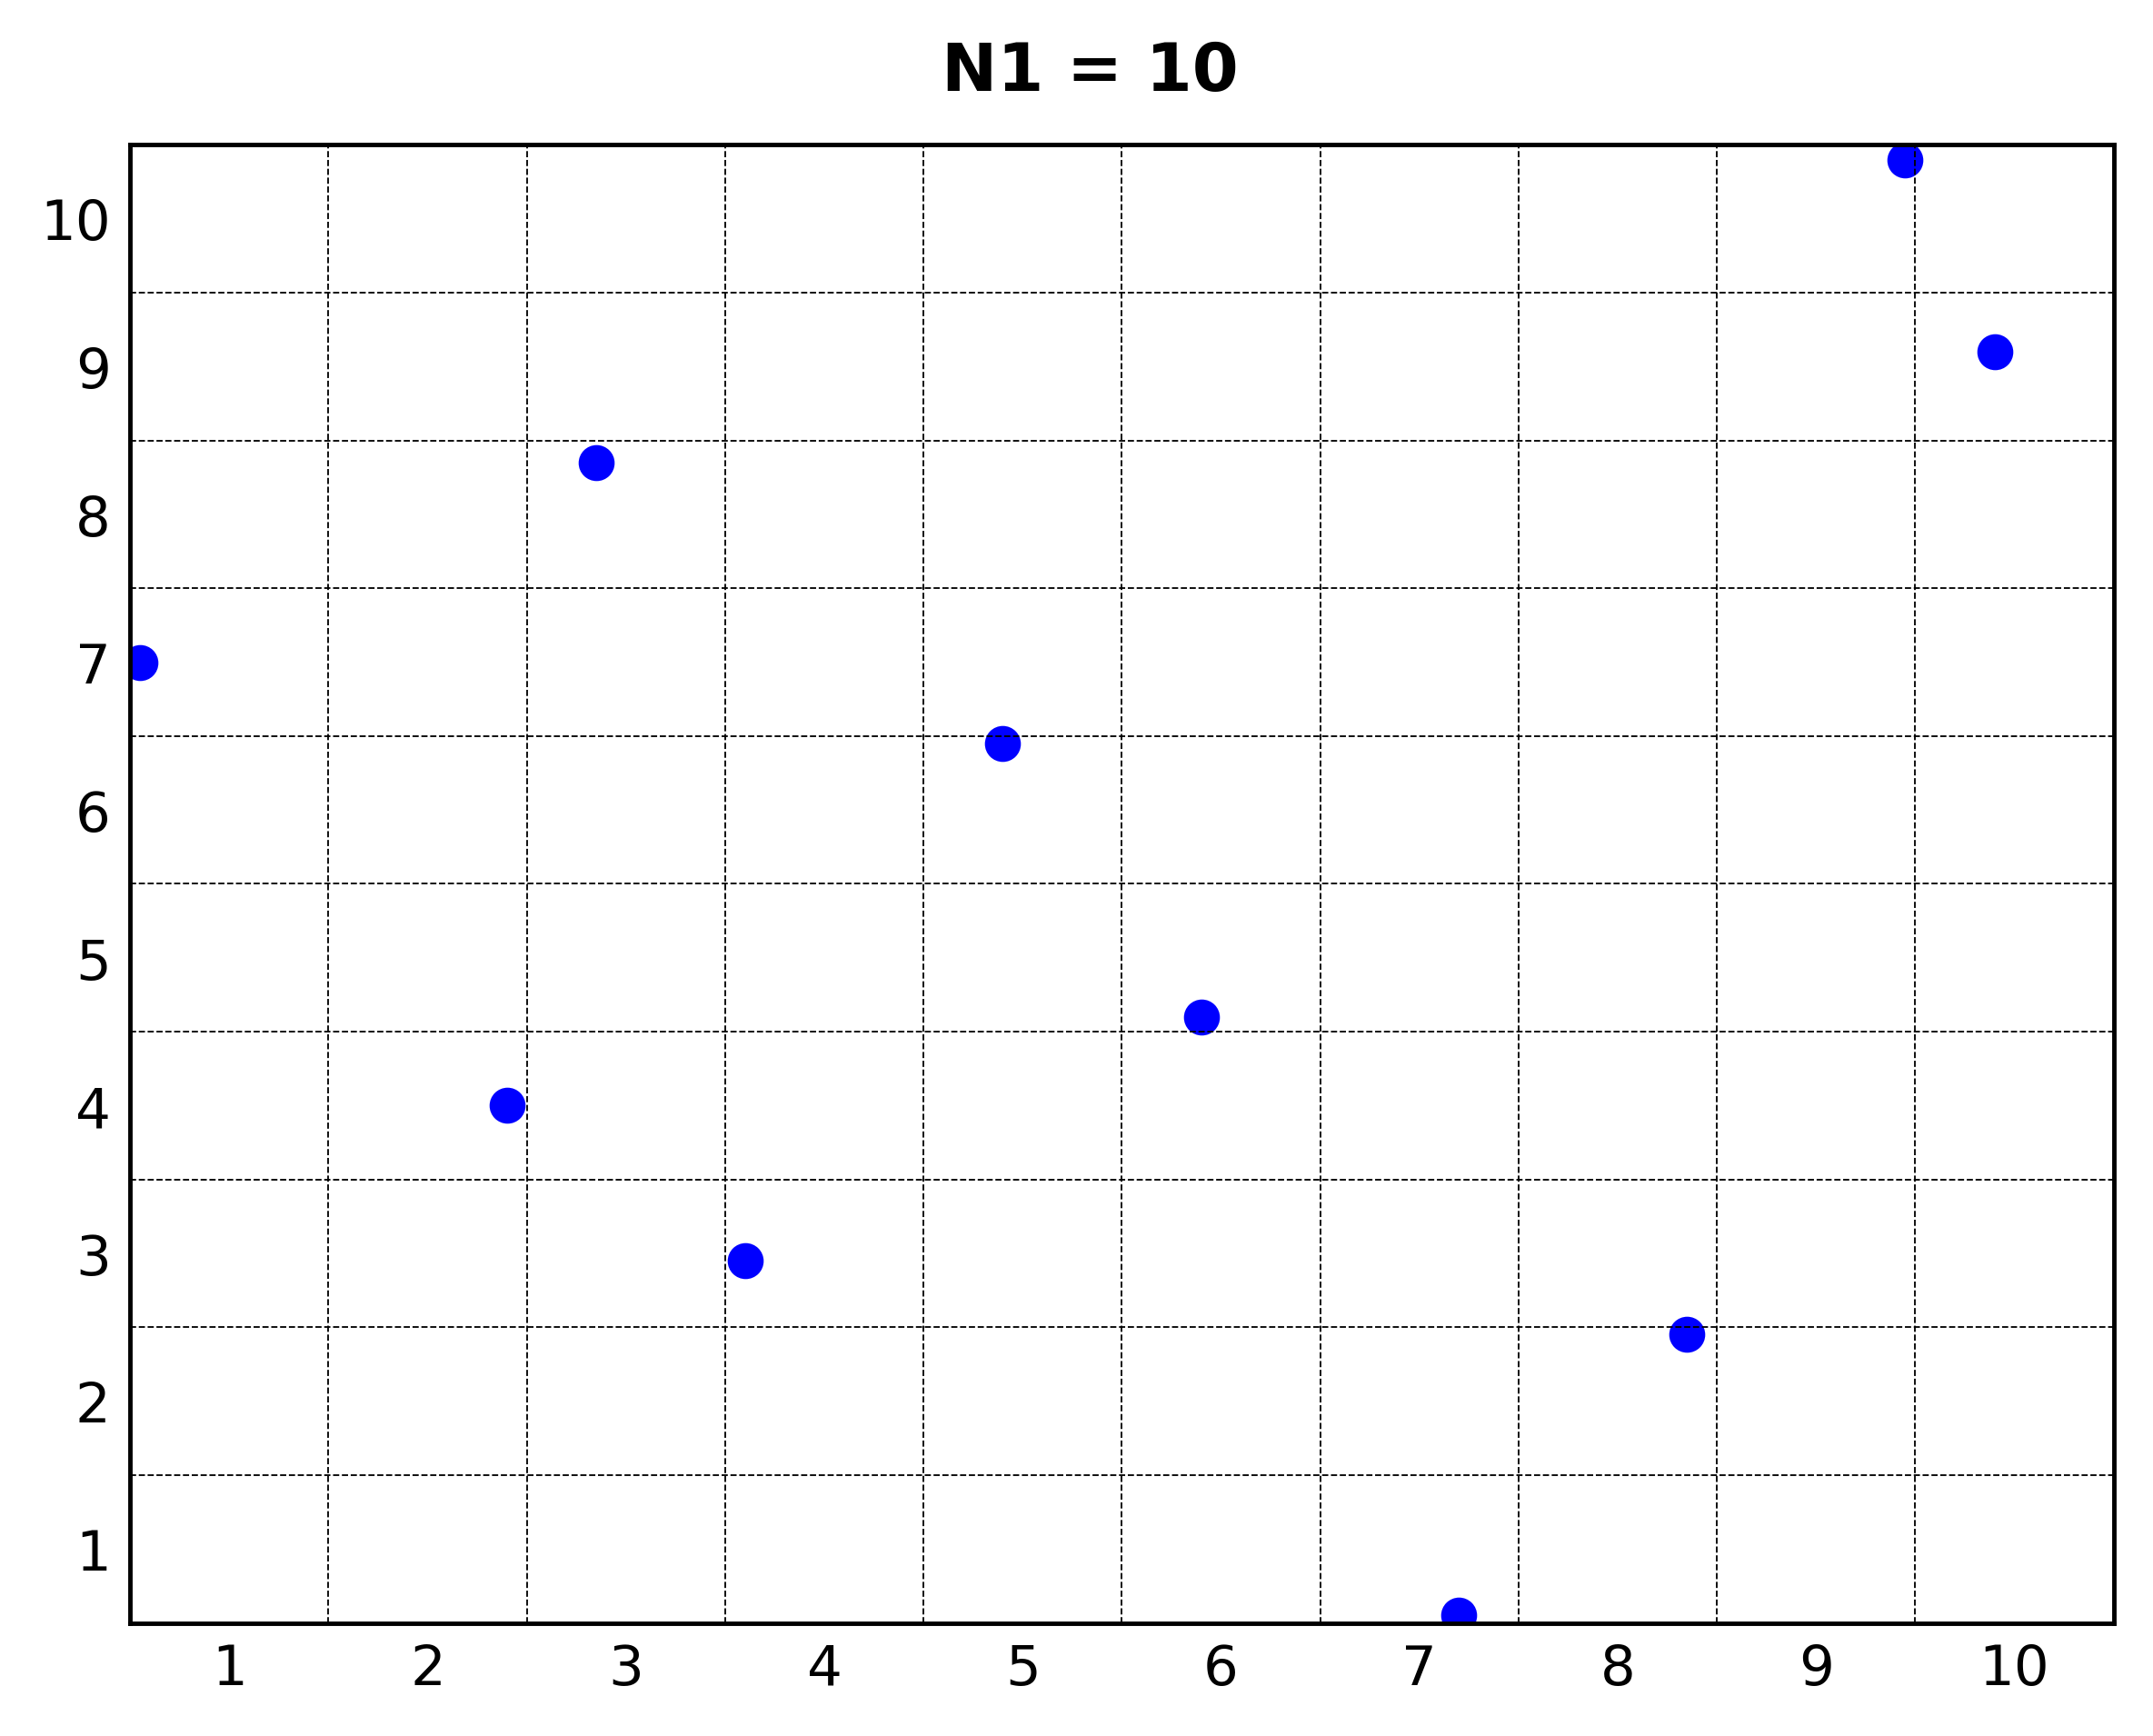
\includegraphics[width=\textwidth]{src/imgs/example_overlaps1.png}
        	\label{fig:example_overlaps1}
        }
    \end{subfigure}
    %\hspace{0.05\textwidth}
    \begin{subfigure}[b]{0.49\textwidth}
        \centering
        \vtop{
        	\vspace{0pt}
        	\captionsetup{skip=0pt}
        	\midcaption{}
        	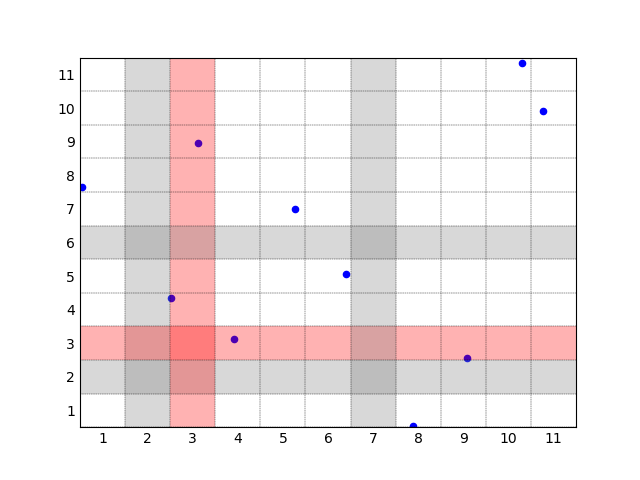
\includegraphics[width=\textwidth]{src/imgs/example_overlaps2.png}
        	\label{fig:example_overlaps2}
        }
    \end{subfigure}
    
    \begin{subfigure}[b]{0.49\textwidth}
        \centering
        \vtop{
        	\vspace{0pt}
        	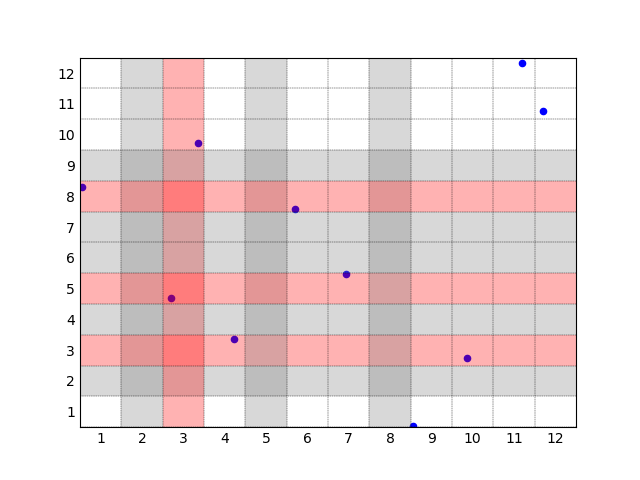
\includegraphics[width=\textwidth]{src/imgs/example_overlaps3.png}
        	\captionsetup{skip=0pt}
        	\midcaption{}
        	\label{fig:example_overlaps3}
        }
    \end{subfigure}
    %\hspace{0.01\textwidth}
    \begin{subfigure}[b]{0.49\textwidth}
        \centering
        \vtop{
        	\vspace{0pt}
        	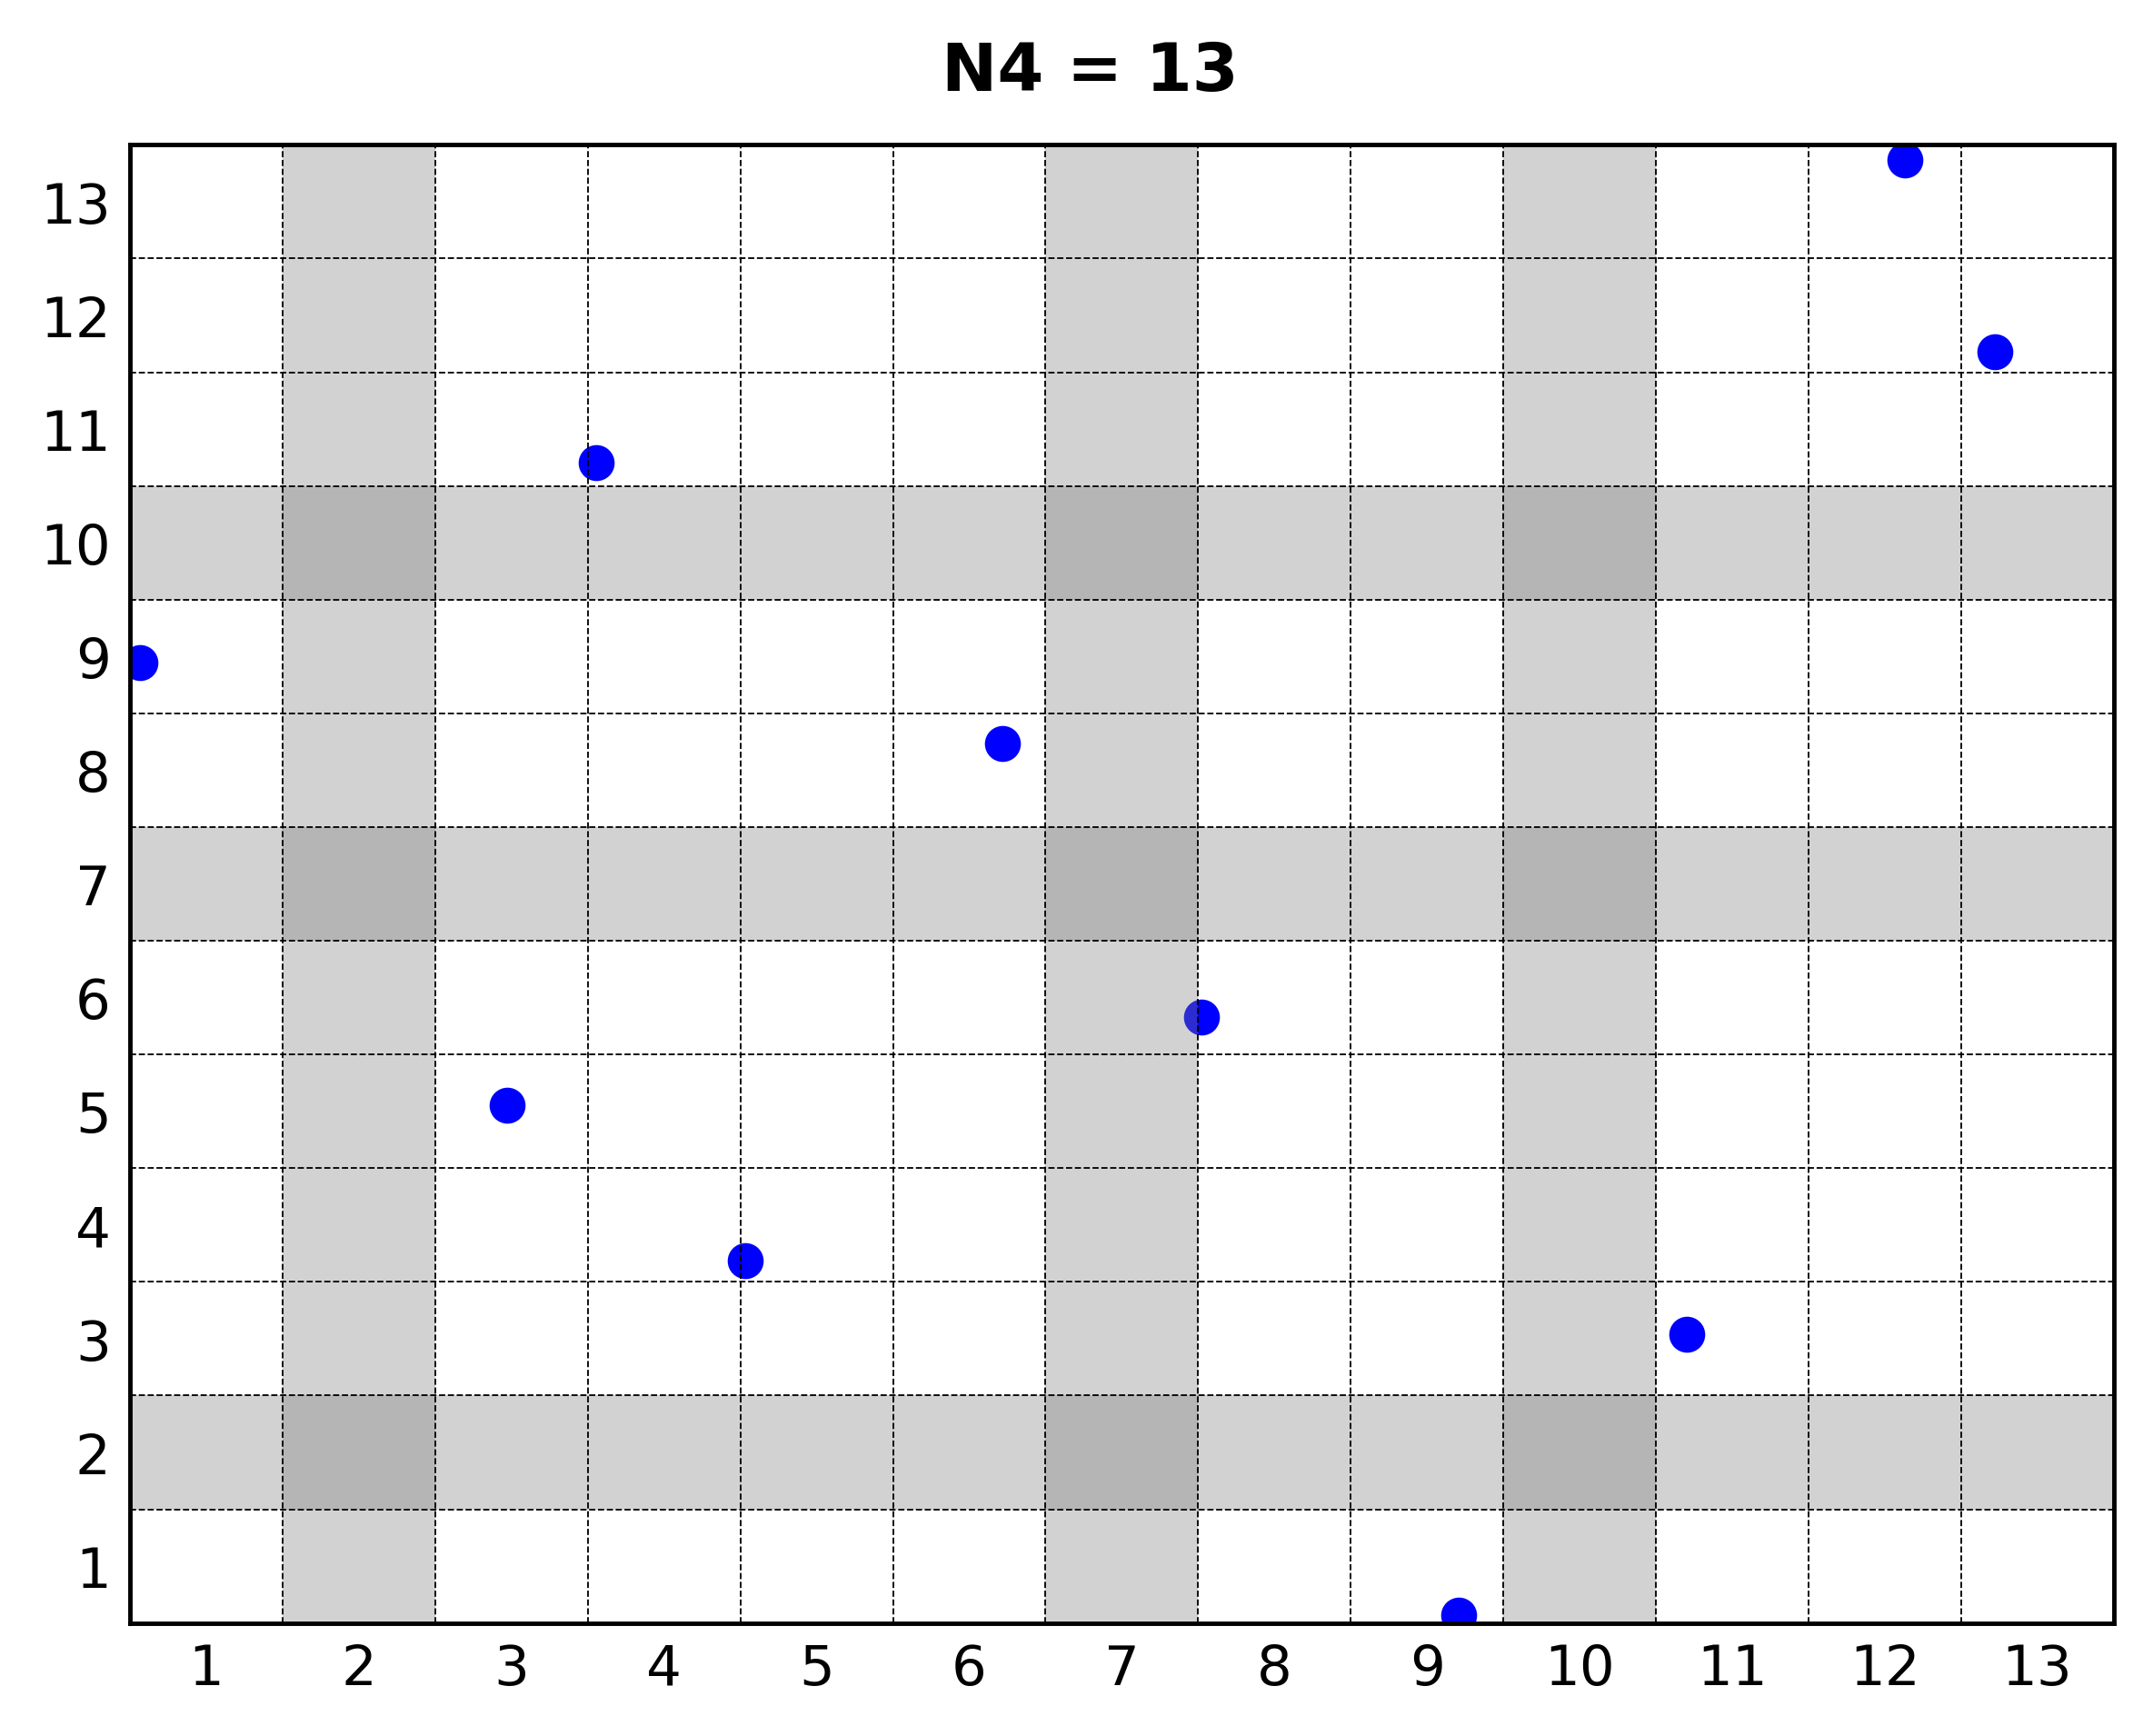
\includegraphics[width=\textwidth]{src/imgs/example_overlaps4.png}
        	\captionsetup{skip=0pt}
        	\midcaption{}
        	\label{fig:example_overlaps4}
        }
    \end{subfigure}
    
    \caption{To demonstrate the behavior of the grid, $S \in LHS(N_1 = 10, P = 2)$ sample set is allocated and projected over the grid as it grows one by one. Rows and columns marked in red indicate the location of overlaps, while light grey-colored rows and columns are vacant. In (a) $N_1 = 10$ LHS samples are displayed over a grid of $N_1$ intervals per axis; (b) shows the first step of the growing grid: two overlaps occur in the horizontal and vertical intervals \#3, two intervals per dimension are vacant one of which derives from the expansion vacancy and the other one is caused by the overlap; (c) samples displayed over $N_3 = N_1 + 2$ grid: on the vertical axis there are 3 overlaps and 2 (from the expansion) + 3 (from the overlaps) vacancies; (d) the grown $N_4 = N_1 + 3$ grid have no collisions, then $S$ is a perfect expansion with $M = 3$ expansion magnitude}
    \label{fig:example_overlaps}
\end{figure}


\subsection{Grade of an Expansion}
\label{subsec:expansion_grade}
A precise heuristic that expresses how near the current expansion is to a perfect expansion, given the desired expansion magnitude $M$ and the beginning state, is necessary for developing a new sample set. Since the metric in \meqref{eq:grade} is no longer sufficient, the variation \textit{expanded grade} has been offered.
The purpose of the \textit{expanded grade} is to convert the sample set $S$ of $N$ elements into an index when the sample set is compared against a $P$-dimensional hypercube grid of $N+M$ intervals per axis - this is where it deviates from \meqref{eq:grade}. Here it follows:

\begin{equation}
\label{eq:expanded_grade}
gr(S, M) := \frac{\sum^P_{j=1}\sum^{N + M}_{q=1} min(\sum^N_{i=1}\indfunc{[\frac{q-1}{N + M}, \frac{q}{N + M})}(S_{ij}), 1)}{P \cdot (N + M)}
\end{equation}

Each $I$ interval contributes to \meqref{eq:expanded_grade} value with a share of:

\begin{equation}
\label{eq:single_contribute_interval}
\mu_I = 
\begin{cases}
\frac{1}{P \cdot (N+M)} \qquad \text{\textit{if any x $\in$ I}}\\
0 \qquad\qquad\;\;\; \text{\textit{otherwise}}
\end{cases}
\end{equation}

which makes \meqref{eq:expanded_grade} a discrete quantity that ranges from $\frac{1}{N+M}$, if every sample of a non-empty set lies in one single interval per axis, to 1, which represents the perfect LHS expansion.

A perfect expansion for $S \in MC(N, P)$ over a $N+M$ space grid of a number $M$ of intervals (per dimension) empty, given that, by definition of LHS, $N$ samples fall in $N$ distinct intervals (per dimension). Then, the only valuable \textbf{$\mu$} shares are given by $N$ intervals while the other $M$ set of intervals are empty. From this statement, we can provide an upper limit for the expanded grade by starting from 1 - the maximum possible index of a perfect LHS sample set - minus the total weight lost during the growing of the grid, which corresponds to the total number of \textit{voids} times \meqref{eq:single_contribute_interval}. The total number of \textit{voids} is equal to $M \cdot P$ because they are evenly spread across each dimension. So, $Z$ is a \textit{perfect expansion} of $S$ with $M$ additional intervals if and only if:

\begin{equation}
\label{eq:upper_limit_perfect_expansion}
gr_{max}(S, M) = 1 - \frac{M}{N+M}
\end{equation}

The \textit{initial set} $S \in MC(N, P)$ plotted over $P$ hypercube of $M+N$ intervals (per dimension) is called \textit{perfect expansion} if and only if $S$ expanded grade \meqref{eq:expanded_grade} is equal to the \textit{upper expanded grade limit} \meqref{eq:upper_limit_perfect_expansion}. \\
As the name may suggest, the perfect expansion is the best possible candidate to produce an optimal non-collapsing sample set, so an LHS, as result of an expansion process described in \cref{subsubsec:general_expansion_case}.


\subsection{The expansion process}
The expansion task was initially handed at the very beginning of  \cref{subsec:multistage_task} as a evolutionary process which augments the $S$ starting sample set to a next-stage state with increased number of elements $M$, placed as better as it can to maximize criteria. However, we show in \cref{subsec:expansion_grade} that an expansion may demote the non-collapsing property of the resultant expanded set $Z$, which can be measured with the metric \meqref{eq:expanded_grade}. 
In this section the authors propose how to place the new samples to achieve maximum "LHS-ness" over any $M$ expansion magnitude needed and introduce its potentialities for future researches - see more in \cref{sec:conclusions}.

In first place, the proposal is delivered by studying the basic case of a perfect expansion in \cref{subsubsec:perfect_expansion_case}, then extend to the general case with any non-perfect expansion outcome.

\subsubsection{State case - Perfect Expansion}
\label{subsubsec:perfect_expansion_case}
An initial instanced sample set $S$ of $N$ elements can be perfect expanded if and only if $S$ after the $M$-th growing step of the $P$-hypercube grid has the maximum grade (\meqref{eq:upper_limit_perfect_expansion}). Furthermore, \mfigref{fig:example_overlaps4} well depicts what the experimenters would expect before setting down an expansion set $E$. We notice the best candidate extent is likely the empty intervals (in light grey) because they do not interfere with other well-formed intervals. It is also imperative that the new samples do not overlap onto each other over the vacant space (\textit{vacancies} or \textit{voids}, as we previously called them).

First of all, it's necessary to trace each void's index. Here it comes into use again the permuted index matrix, previously used in \cref{subsec:how_to_lhs} to scatter the samples across the hyper-parameter space. The matrix of voids $P \times M$ is composed by the row vectors: 

\begin{equation}
\label{eq:voids_matrix}
\textbf{V}_j = \bigg( q : \nexists\; x \in S_{ij} \; s.t. \; x \in \Big[\frac{q-1}{N+M}, \frac{q}{N+M}\Big) \bigg) \quad, \quad \forall j = 1...P
\end{equation}

which should be element-wise permuted along each row to prevent \mfigref{fig:diagonal_poor_design} diagonalized situation.
Then, the expansion set $E$ collects all the newly generated samples which are a distribution likewise \meqref{eq:rand_variable_Sij} but using $V_{ji}$. 

In the end, the initial $S$ set is concatenated with expansion set $E$, originated from the voids of the $N+M$ growing grid, in a perfect expansion, that guarantees the fulfilling of the non-collapsing property (grade = 1). 

A perfect expansion is a intuitively rare event: each sample has to avoid overlaps. This could eventually happen if two sample projections are spaced more than $\frac{1}{N+M}$ apart (new size of the intervals), But if they are closer, another condition has to be fulfilled: for any $M$ close enough to $N$, a \textit{critical span} exists across the \textit{i-th frontier} (see right after \meqref{eq:interval_index} for definition) - which shares its boundary with the next interval. The critical span is the intersection area between two neighbor samples intervals and the eventual interval raised across them (\mfigref{fig:critical_span2}). Given that LHS is not supposed to consider further additional points, it might happen that samples are placed in critical areas (after a $M$ growing step). An example of how can a couple of collapsing samples can occur is shown in \mfigref{fig:critical_span}. In the example, the first sample (in \mfigref{fig:critical_span2}) has been generated in the critical area that is the intersection between \textit{$\sim$2} and \#1 original interval. On its hand, the second sample lies upon the same critical area between \textit{$\sim$2} and \#2 original subspace. Hence, in the example the two samples are overlapped.

\begin{figure}[h]
    \centering
    \begin{subfigure}[b]{0.45\textwidth}
        \centering
        \vtop{
        	\vspace{0pt}
        	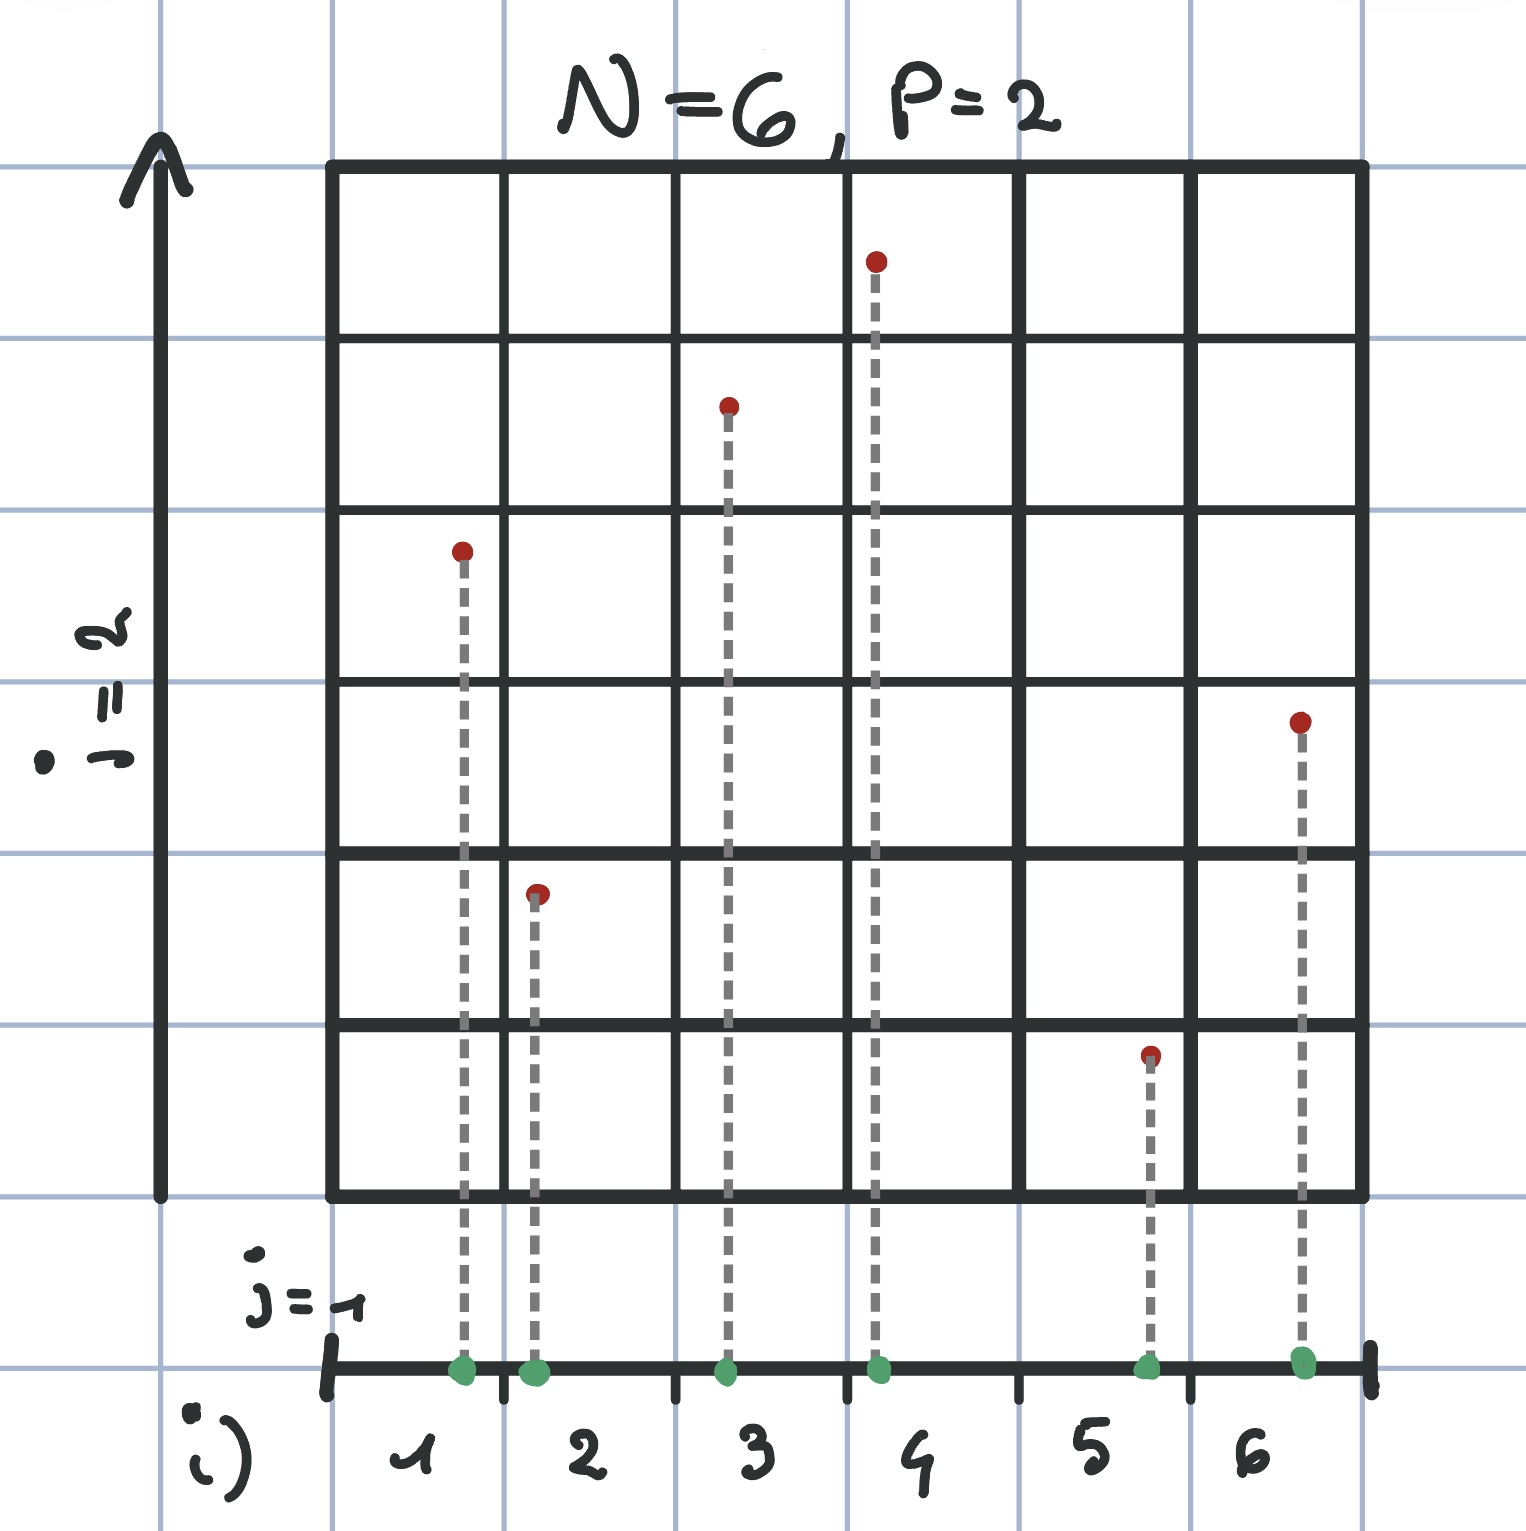
\includegraphics[width=\textwidth]{src/imgs/critical_span_init.jpg}
        	\caption{An LHS of $N = 6$ samples expanded for $M = 2$. on the horizontal axis are projected the horizontal component of all samples. [SKETCH - ne farò in digitale di migliori]}
        	\label{fig:critical_span1}
        }
    \end{subfigure}
    \hspace{0.05\textwidth}
    \begin{subfigure}[b]{0.45\textwidth}
        \centering
        \vtop{
        	\vspace{0pt}
        	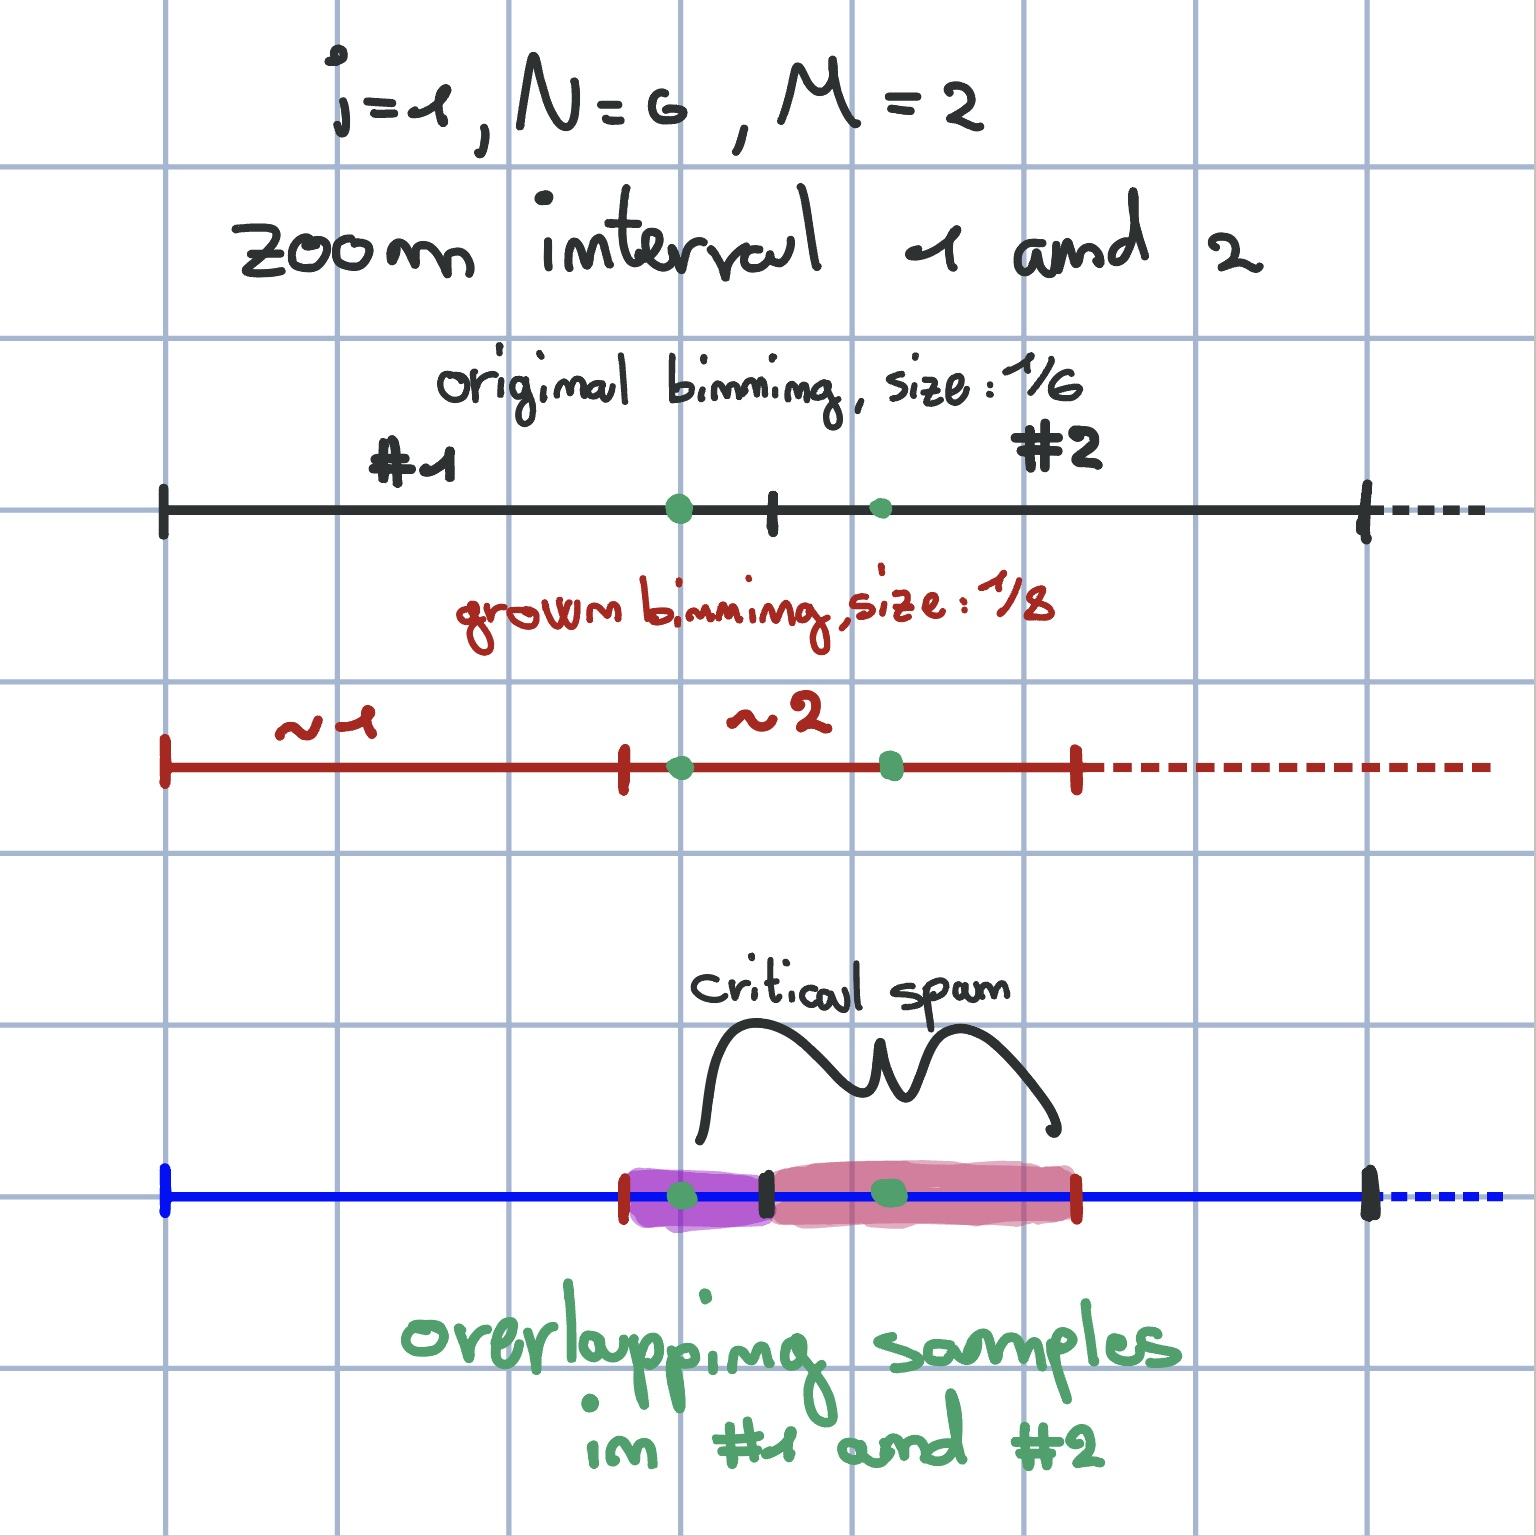
\includegraphics[width=\textwidth]{src/imgs/critical_span_zoom.jpg}
        	\caption{Zooming in \#1 and \#2 interval, it's show how both shares a critical area (on the bottom) whereof each one may have been distributed in it. [SKETCH - ne farò in digitale di migliori]}
        	\label{fig:critical_span2}
        }
    \end{subfigure}
    \midcaption{ }
    \label{fig:critical_span}
\end{figure}
 
The number and displacement of overlaps and vacancies are pretty hard to predict: they are strongly correlated to the \meqref{eq:Sij_def} sample random distribution. However, we experimentally observed that some expansions are peculiar: exactly all expansions with multiples of $N$ are always perfect. That's because critical spans - again, that are given by the intersection of the specific new intervals that cross the old frontiers with the previous intervals - are always void. Take \mfigref{fig:critical_span2} but with grown binning size equals to $\frac{1}{12}$ instead of $\frac{1}{8}$ (so, with $N = 6$ then $M = 12$): new intervals divide perfectly the old ones, without ever crossing any frontier. This concept is properly explained in \mappendixref{appendix:N_multiples}. Explicitly:

\begin{equation}
\label{eq:known_perfect_expansions}
\forall K \in \mathbb{N}^+ \;\; : \;\; S \in LHS(N, P) \Rightarrow gr(S, K \cdot N) = gr_{max}
\end{equation}

[I'm not exactly sure if it should be $\Rightarrow$ or $\Leftrightarrow$]

\subsubsection{State case - General Expansion}
\label{subsubsec:general_expansion_case}
During the upscale of $S$ from $N$ to $N+M$ number of elements, it comes along with a variable number of overlaps on j-th axis $O_j$.
In \cref{subsec:expansion_grade} the authors stress the relation between tuples $\textbf{V}_j$, $M$, and the amount of collisions $O_j$ on each j-th dimension. Specifically:
\begin{equation}
\label{eq:vjojm}	% nome norvegese di alto rango
\parallel \textbf{V}_j \parallel = O_j + M
\end{equation}
whereof the overlaps count equals to zero, the expansion has been perfect (see \cref{subsec:multistage_task}). In a general case of expansion, the overlaps amount is most likely not equal to zero in some dimensions.

The case study implies that the creation of the expansion set i$E$ is not trivial anymore because of the irregularity of the vacancies set. By referring to \meqref{eq:vjojm}, unlike what was stated before, $V$ would probably be no matrix at all but, instead, a set of heterogeneous tuples. If $V$ components was homogeneous, it would have been a inherited matrix. The number of $\textbf{V}_j$ interval indexes would likely be more than $M$ sample's projections to commit. The expansion algorithm has to pick up a reasonable subset of $M$ void entries, and thus to discard an amount of intervals equal to the number of overlaps $O_j$. Therefore, given the sub-hyperspace settled by the joined selected voids, in order to plot an $M$ amount of new samples, it will pick up an $P \times M$ submatrix (that mimics \meqref{eq:voids_matrix}) of $V$ set. The submatrix should be handled being aware that it would effect the samples layout which may better improve another coherent criteria chosen (such as low-discrepancy or Maximin space-filling).\\
The selection process of vacancies from an irregular $V$ voids set is described by a function $\sigma: N \times P, \; M \rightarrow P \times M$, namely \textit{perfectify} or \textit{vacancy reduction} (for the matter of giving names to anything). \\ 
In this section, $\sigma$ reduce function trivially picks up $M$ intervals randomly per dimension and build up a permuted \meqref{eq:voids_matrix} vacancies matrix, which will be plugged into \meqref{eq:Sij_def} to produce an expansion set. 

In other words, $\sigma$ criterion extracts from each j-th axis of the vacancies set $\textbf{V}_j$ a fixed $M$ number of elements which are going to compose the sub-hyperspace where $M$ samples will be placed using at least the non-collapsing property. The function $\sigma$ discards $O_j$ number of intervals (\meqref{eq:vjojm}), then creating an amount of voids of the same quantity. Hence, the number of overlaps $O_j$ determines the number of void intervals after the expansion is consumed.

In this paper, the term \textit{quasi-LHS} refers to a non full-graded in-th stage of expansion descended from a proper LHS.

\begin{figure}[]
    \centering
    \begin{subfigure}[b]{0.45\textwidth}
        \centering
        \vtop{
        	\vspace{0pt}
        	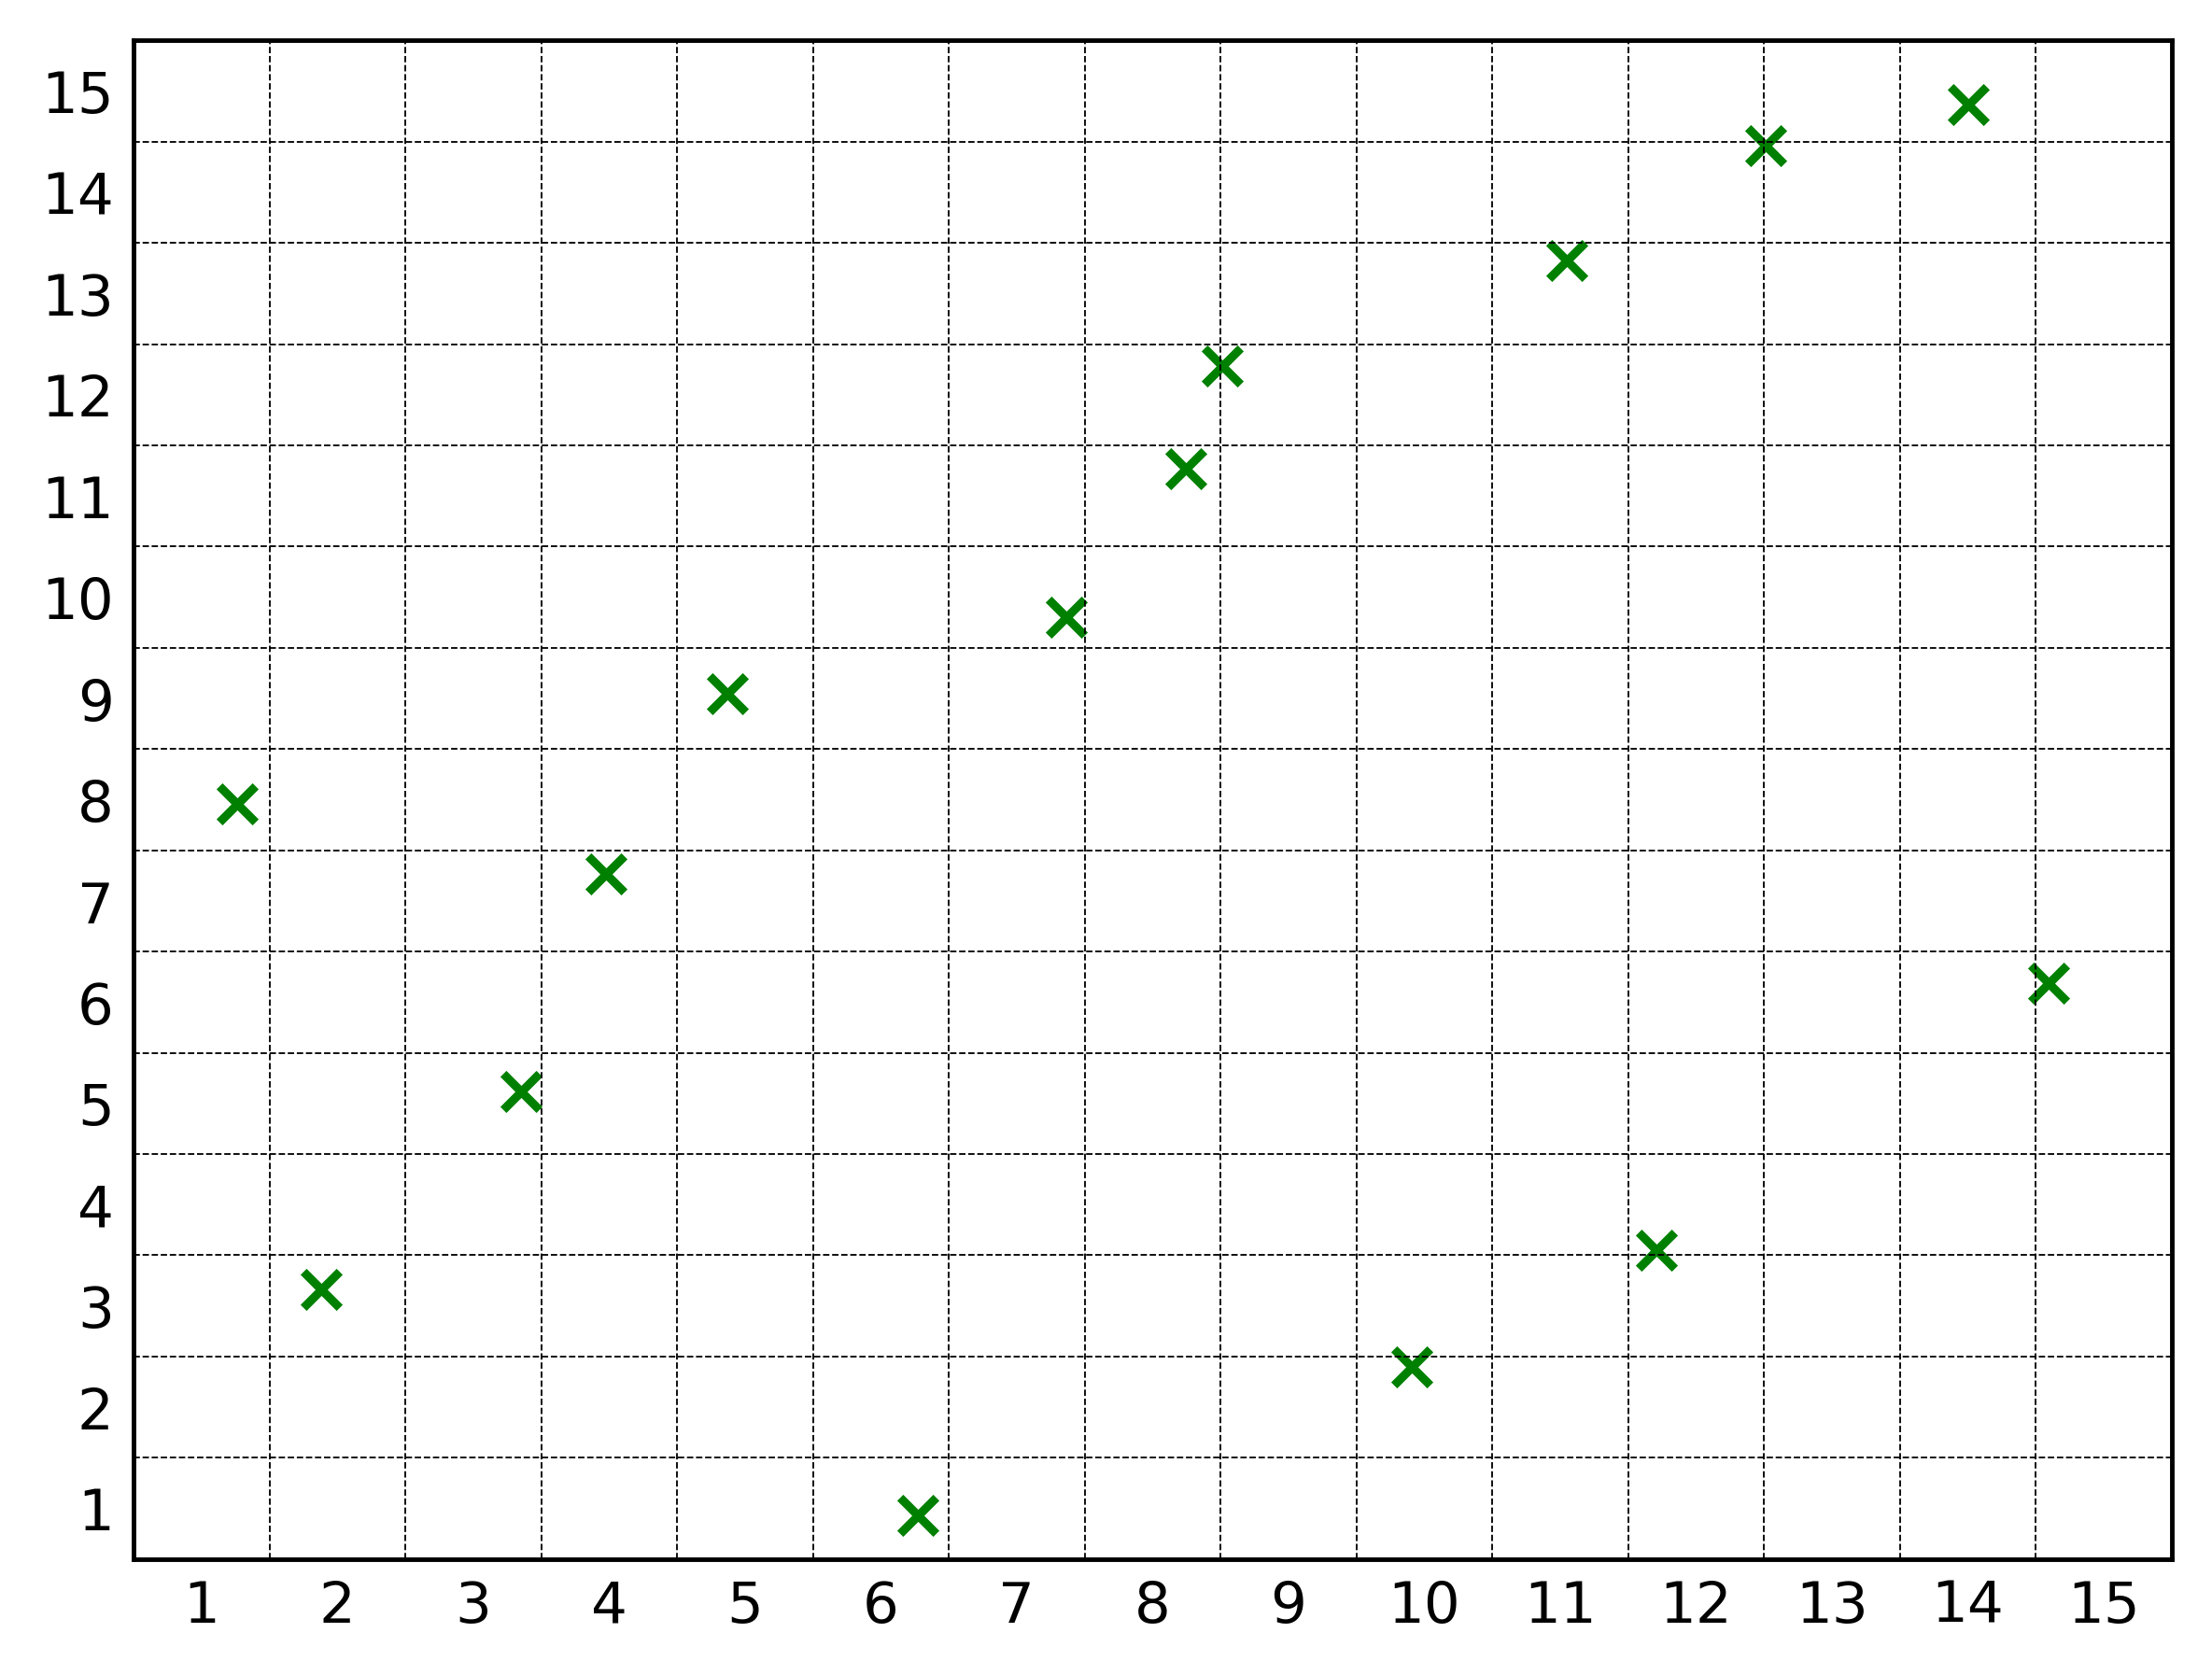
\includegraphics[width=\textwidth]{src/imgs/algo1.png}
        	\captionsetup{skip=0pt}
        	\caption{First-stage LHS of $N = 15$ samples in $P = 2$ generated with scipy's qmc library.}
        	\label{fig:algo1}
        }
    \end{subfigure}
    \hspace{0.05\textwidth}
    \begin{subfigure}[b]{0.45\textwidth}
        \centering
        \vtop{
        	\vspace{0pt}
        	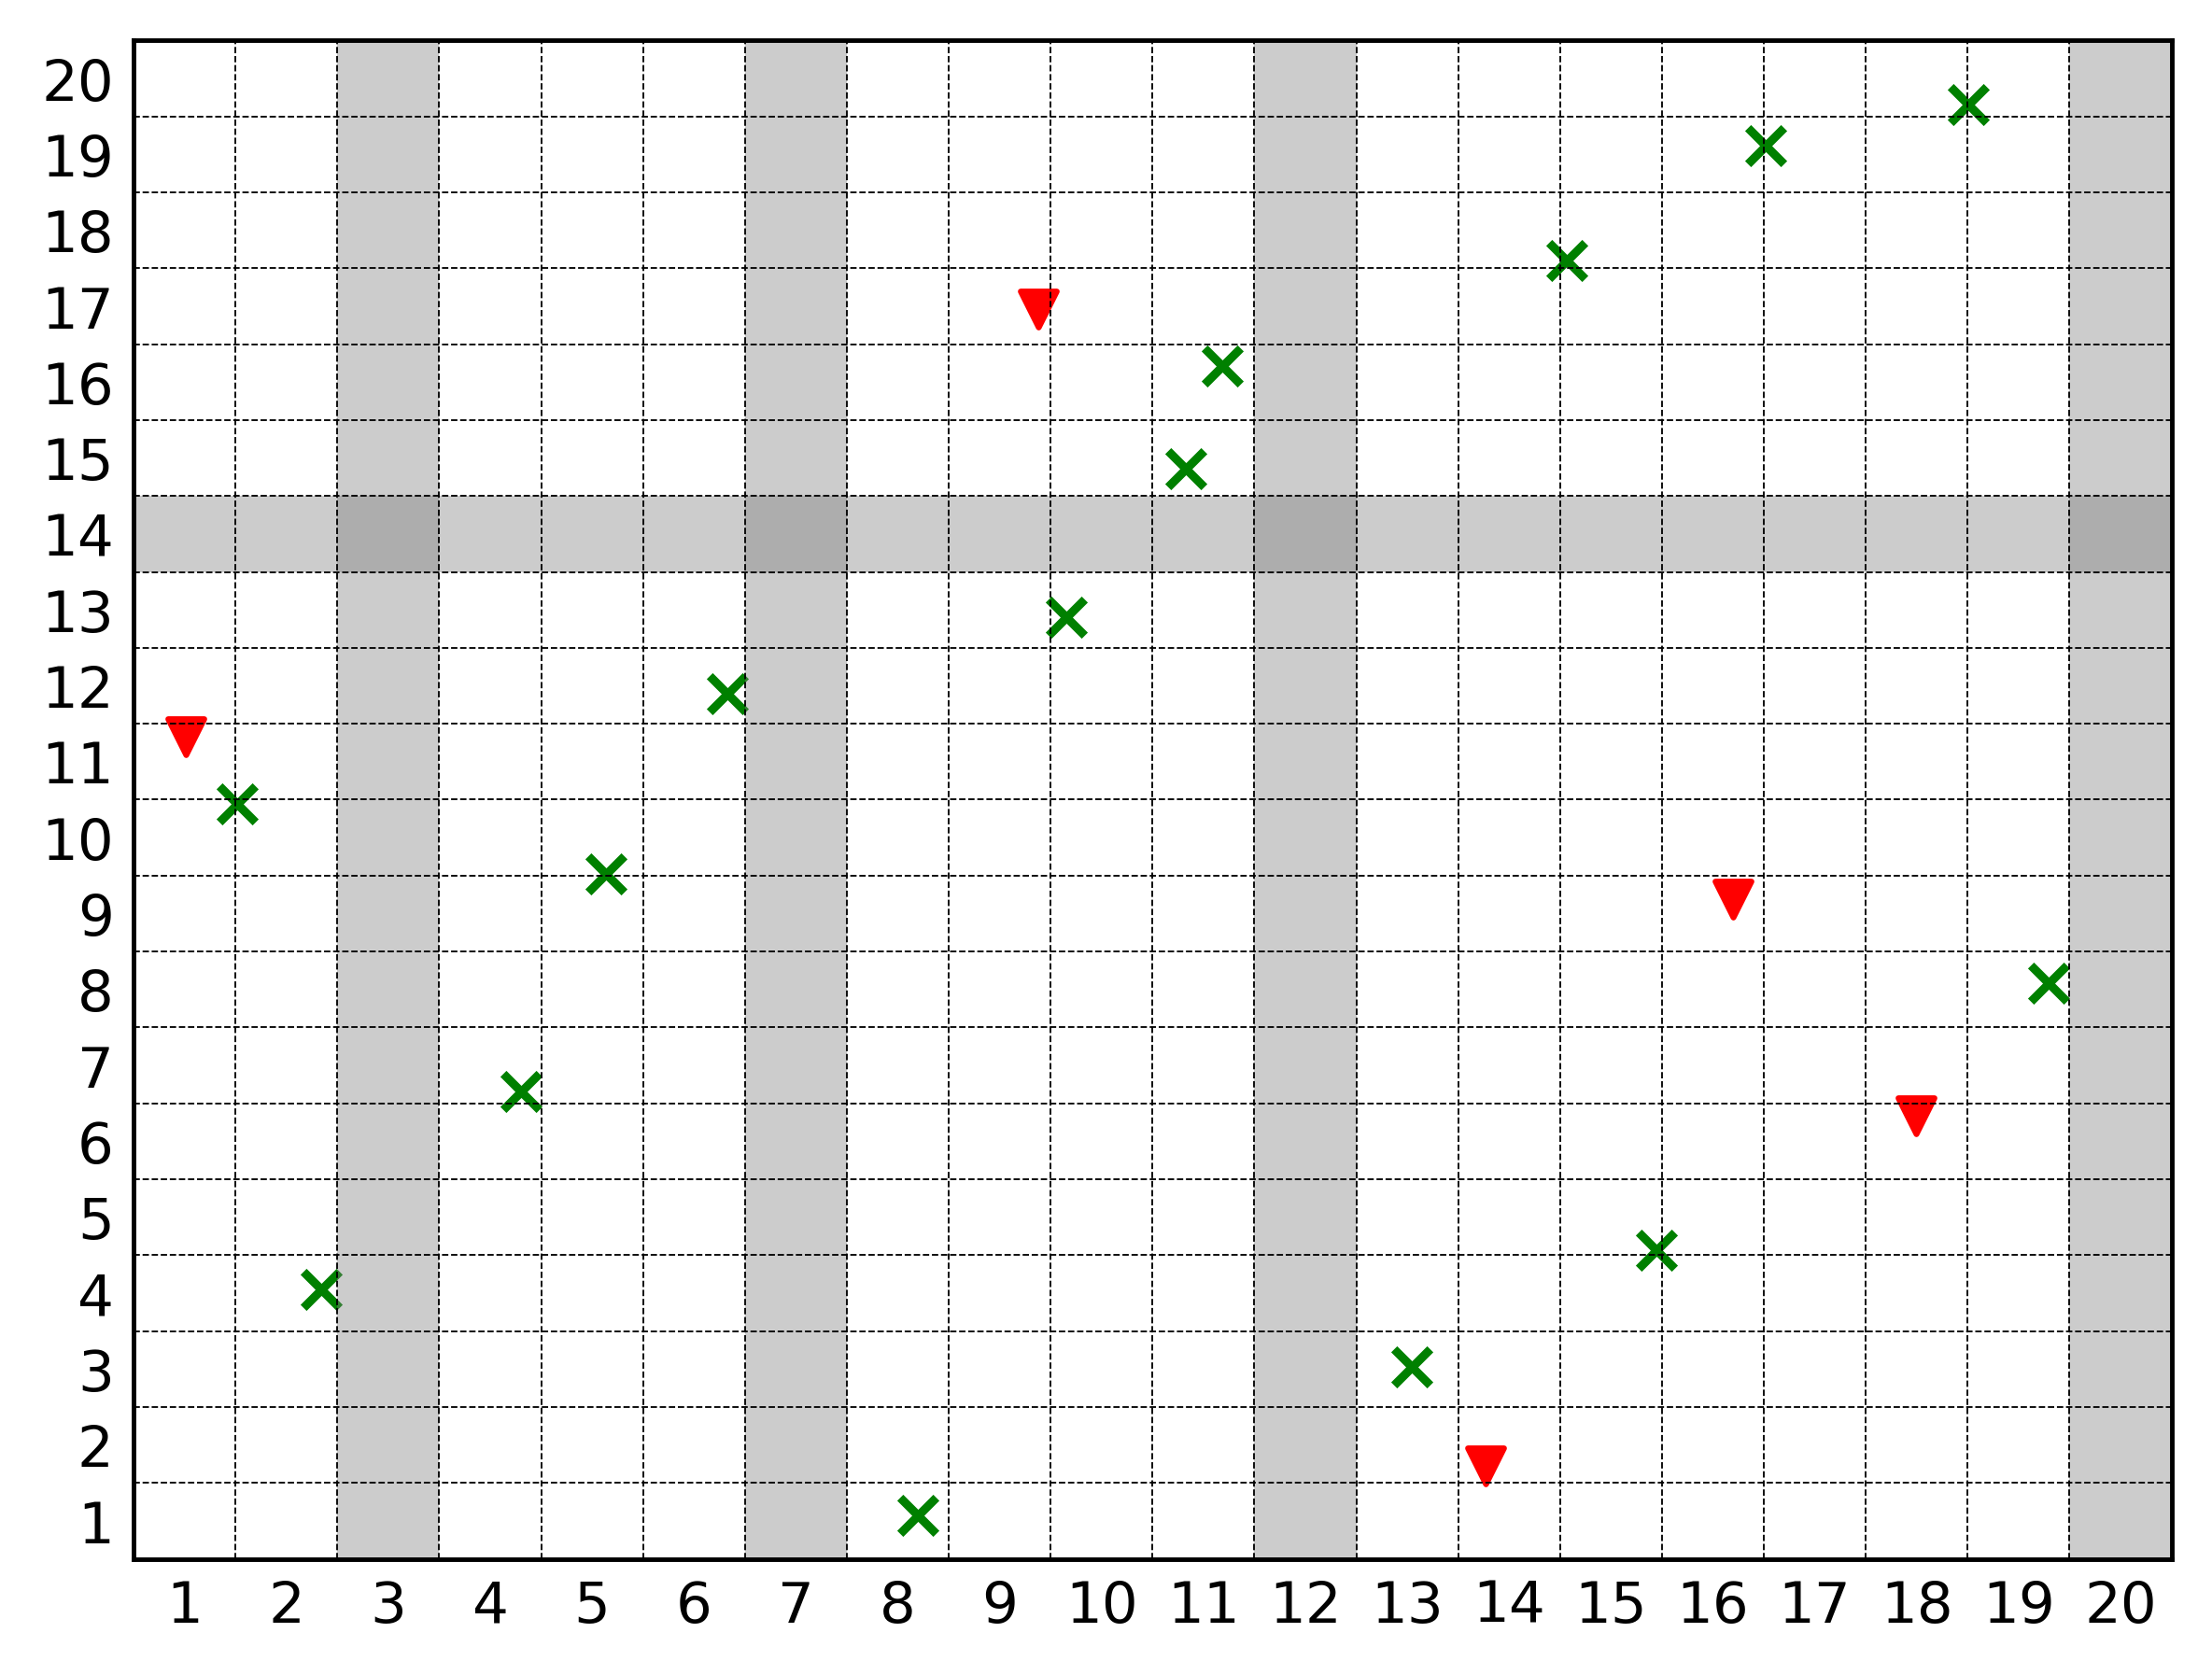
\includegraphics[width=\textwidth]{src/imgs/algo4.png}
        	\captionsetup{skip=0pt}
        	\caption{Expansion of (a)'s LHS with \cref{subsubsec:algorithm} eLHS algorithm given $M = 5$ new samples. Note that the light grey marked intervals are empty and, according to \cref{subsubsec:general_expansion_case}, they are related with the overlaps distribution in (c)}
        	\label{fig:algo2}
        }
    \end{subfigure}
    \captionsetup{justification=centering}
    \caption*{Above is shown a two-staged quasi-LHS. (a) is the first original LHS and (b) is next stage expansion of it.}
    
    \begin{subfigure}[b]{0.45\textwidth}
        \centering
        \vtop{
        	\vspace{0pt}
        	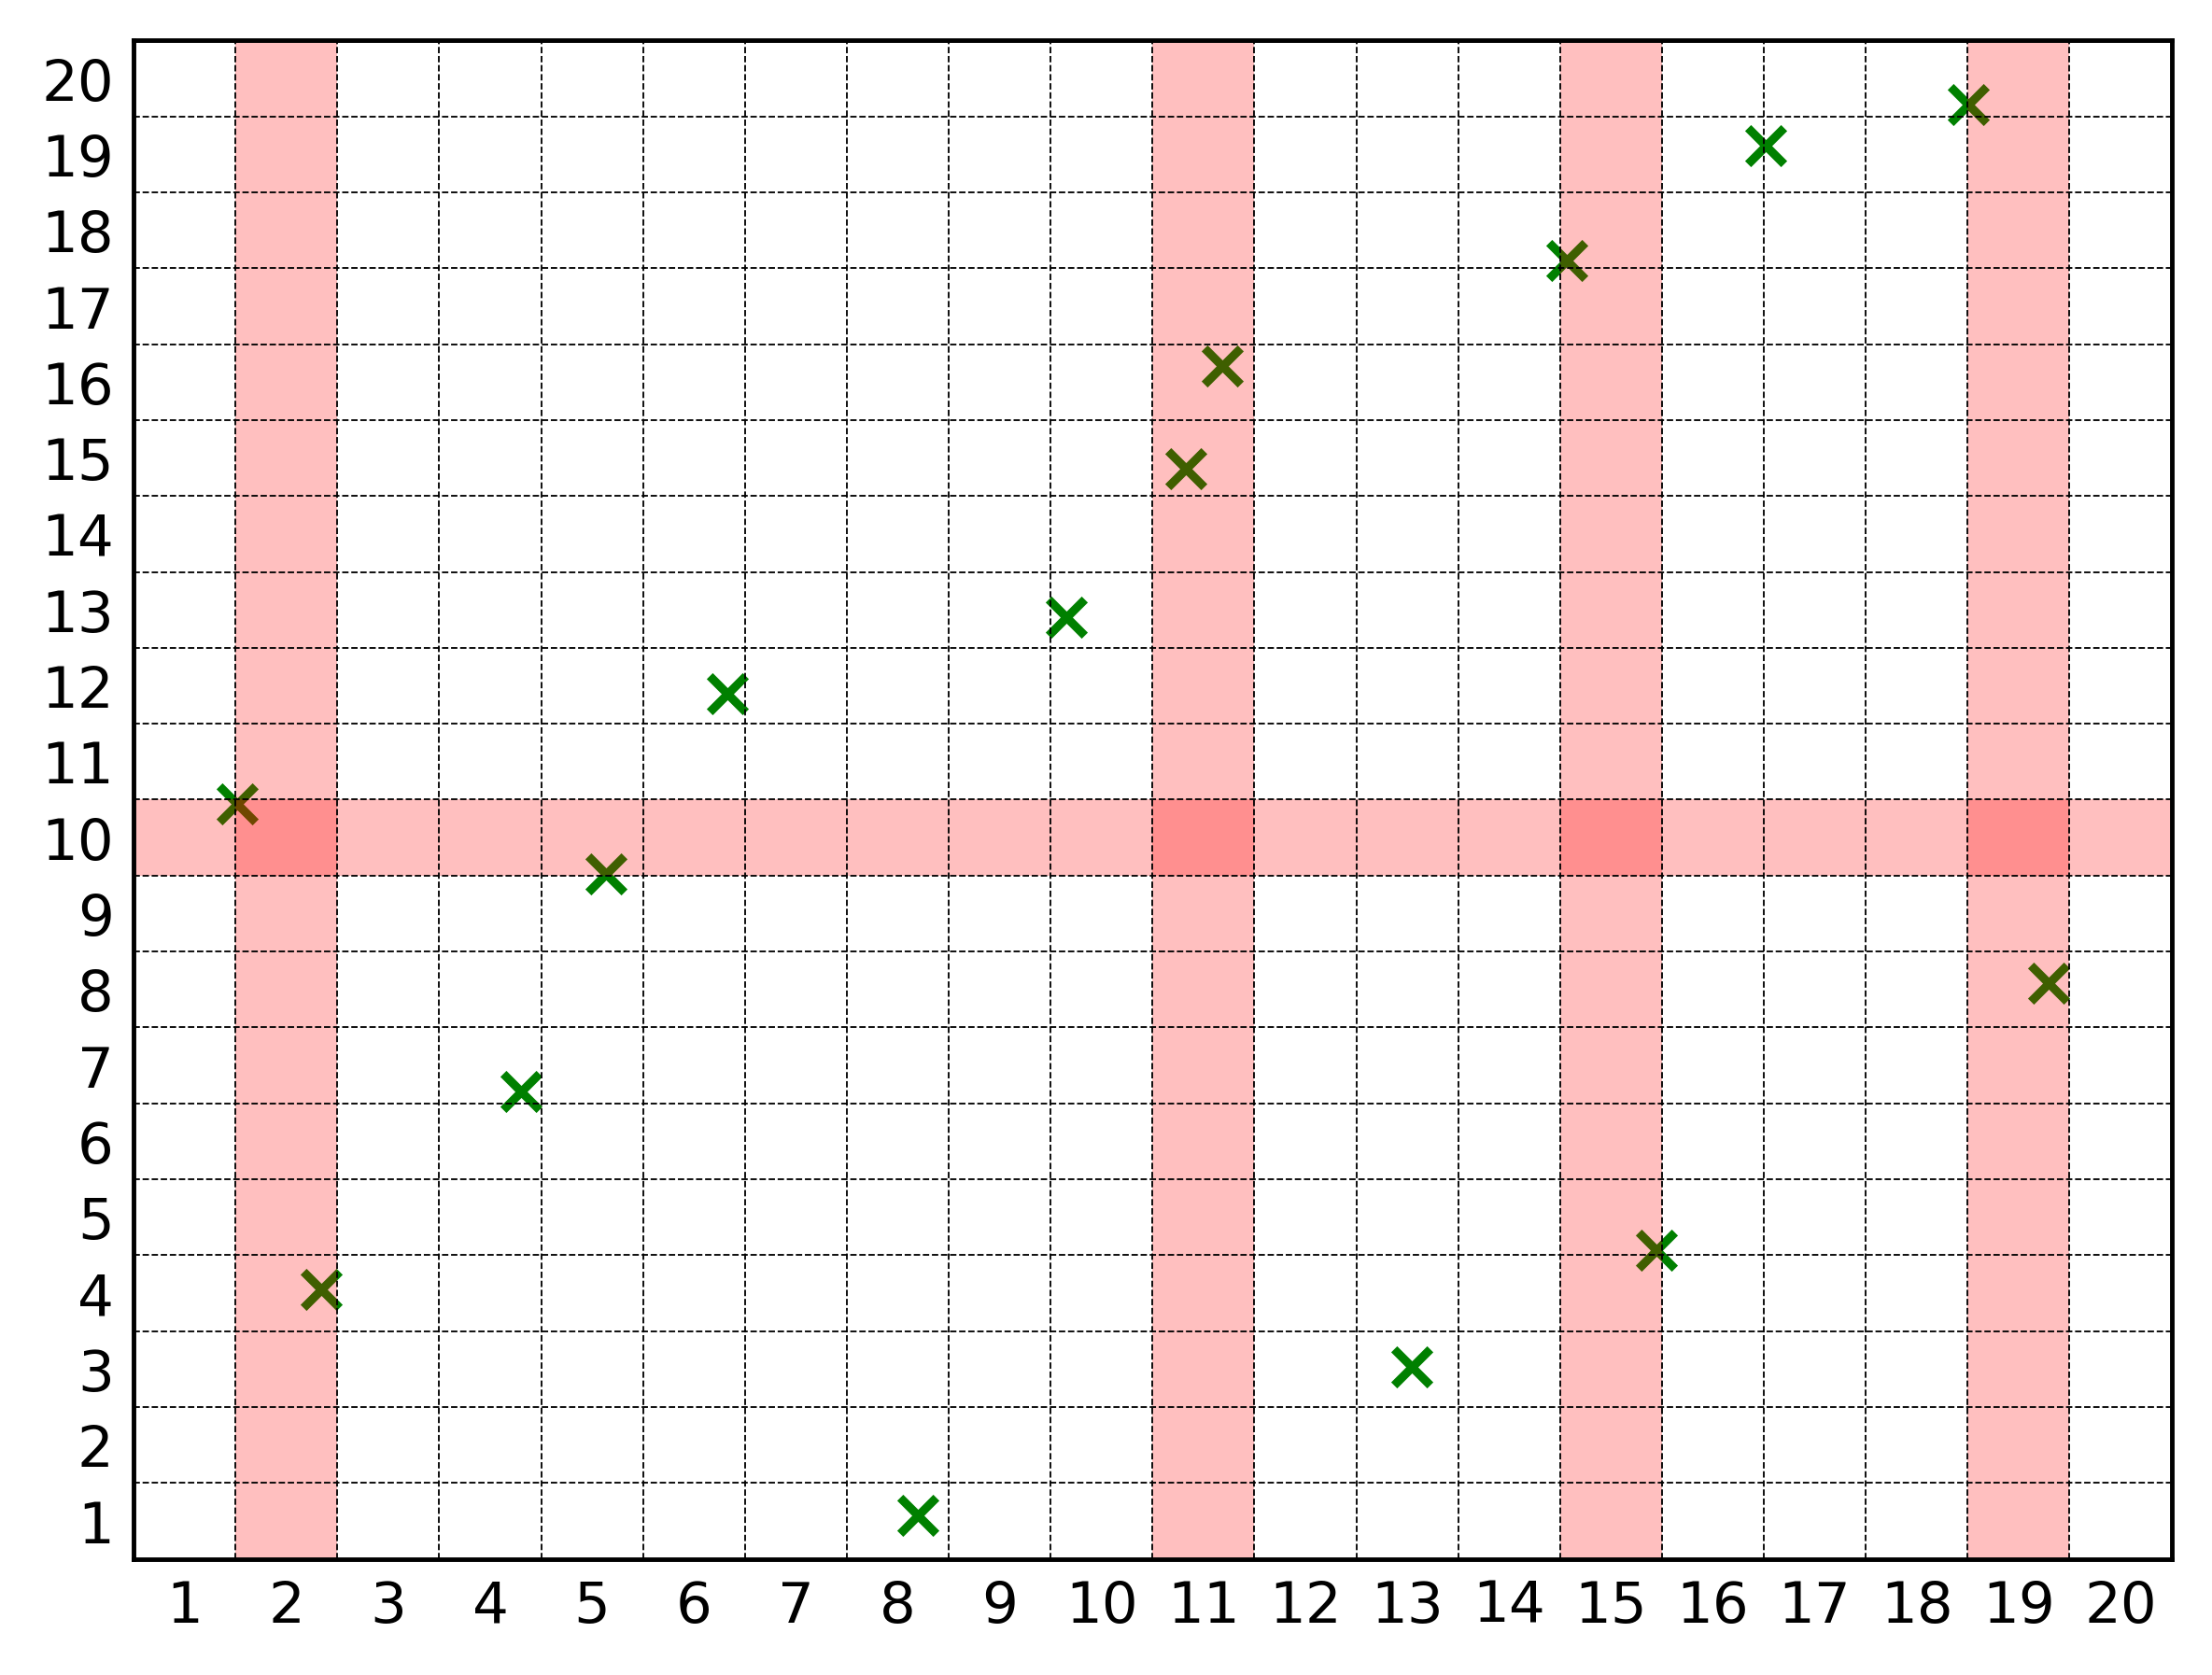
\includegraphics[width=\textwidth]{src/imgs/algo2.png}
        	\captionsetup{skip=0pt}
        	\caption{Red intervals have two sample's projections in it and break the non-collapsing property.}
        	\label{fig:algo3}
        }
    \end{subfigure}
    \hspace{0.05\textwidth}
    \begin{subfigure}[b]{0.45\textwidth}
        \centering
        \vtop{
        	\vspace{0pt}
        	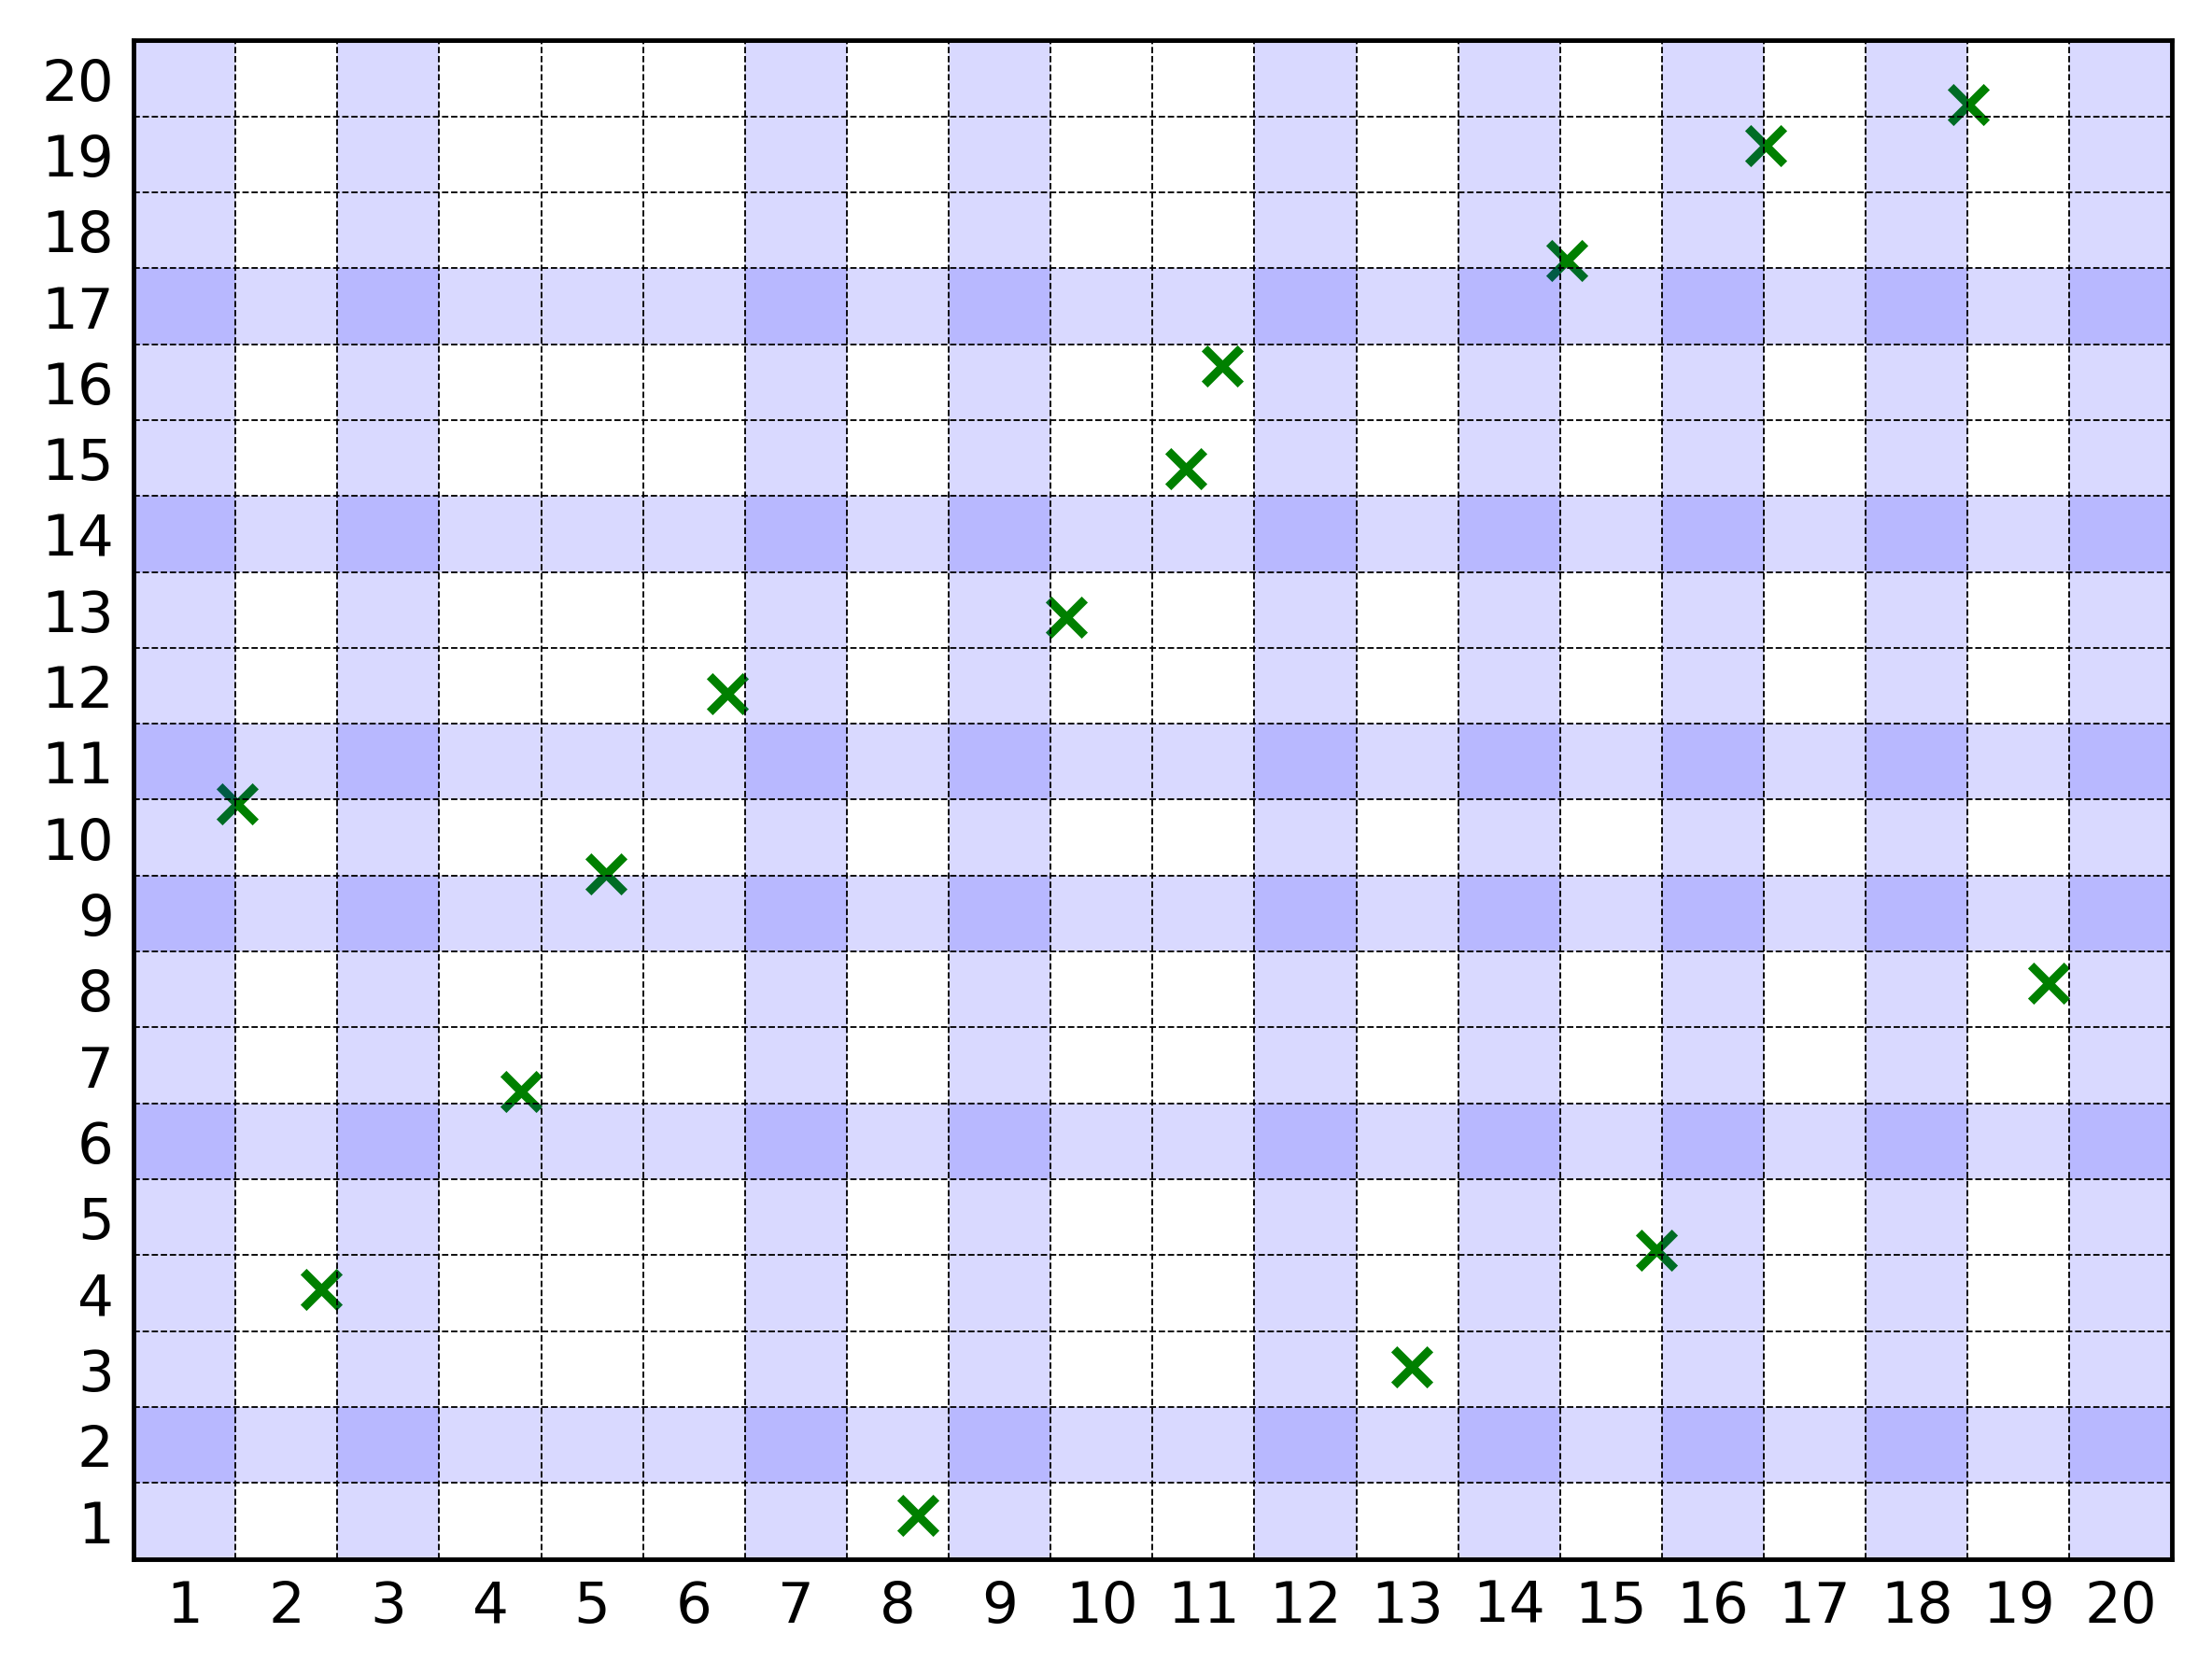
\includegraphics[width=\textwidth]{src/imgs/algo3.png}
        	\captionsetup{skip=0pt}
        	\caption{Blue intervals are empty. They represents the best candidate spots to place new LHS samples. Every interval all together has been referred as the sub-hyperspace of vacancies. }
        	\label{fig:algo4}
        }
    \end{subfigure}

    \captionsetup{justification=centering}
    \caption*{Re-binned (a)'s grid with $N + M$ intervals and plotted against the starting LHS.}
    
   	\midcaption{}
    \label{fig:algo}
\end{figure}

\subsubsection{The eLHS algorithm}
\label{subsubsec:algorithm}
The LHS expansion algorithm, namely \textit{eLHS}, push a starting Latin Hypercube $S$ to the next stage $Z = eLHS(S, M)$ that maximizes at most the non-collapsing property, along with other eventual criterions.

\begin{enumerate}
\item Instance a $V$ vacancies set of $P$ tuples - which may have different lengths (\meqref{eq:voids_matrix}) because every dimension has an arbitrary number of voids (\meqref{eq:vjojm}). The list of all indexes of the $N+M$ grid is filtered accordingly with \meqref{eq:voids_matrix}. \\ 
Visually, the algorithm re-bins the original $S$ grid to achieve $N+M$ intervals. By plotting it against $S$, the reader can visualize where samples overlap and where there are voids.

\item Reduce $V$ vancancies set to a suitable indexes matrix $V^\prime \in Matrix(P, M)$ by extracting from each $\textbf{V}_j$ tuple $M$ elements - which are going to compose the expansion binning grid - using $\sigma$ reduction criteria (see \cref{subsubsec:perfect_expansion_case}). If there are no overlaps (meaning $S$ has maximum expanded grade \meqref{eq:upper_limit_perfect_expansion}) then $V$ is implicitly equal to matrix $V^\prime$, so no reduction criterion is required to be applied. \\
We propose a paradigm which $\sigma$ can be built on. Reduce (abuse of notation) the issue to an harder problem with integer constraints so that solutions are the void interval's indexes. Before generating optimal samples (in step 3.), select the optimal void intervals by considering a trivial "puppet" sample that lies in each possible combination of void intervals. Then apply Branch{\&}Bound methodology [TODO: find good refs for BnB] to find the best integer solution(s).

\item Generate new points over the sub-hyperspace outlined by the permuted $V^\prime$ indexes matrix. Currently, Scipy doesn't implement the instancing of a LHS over a discontinuous space yet.\\
The eLHS' implementers should achieve drawing optimal data from a discontinuous space on their own, based on desired additional criteria and time complexity requirements. However, we suggest the following algorithm structures.
	
\begin{enumerate}
	\item This procedure was inspired by Shang et al.\ucite{shang2021} work based on the pioneering CADEX research (\fancycite{kennard1969}). It was designed to be fast and flexible given some appropriate criteria to optimize:
	\begin{enumerate}

		\item set the variable $\Lambda = M$, iteration index $k = 1$ and initialize the expanded set $E$ empty;

		\item generate $\Gamma_k$ a random pool of, let's say, $\alpha_k$ number of new random sample points. The hyper-parameter $\alpha_k$ should be much greater than $\Lambda$. We would recommend a fast-and-reliable MCS;
	
		\item ignore all points that fall outside $V^\prime$ space;

		\item from $\Gamma_k$ select a subset of optimal samples $\gamma_k$ of $\lambda_k \leq \Lambda$ number of points.
	
		\begin{enumerate}
			\item[$\dagger$] If $\lambda_k = 1$ it is like drawing the very optimal point each iteration;
			\item[$\dagger$] If $\lambda_k > 1$ the algorithm should yield a bunch of samples which satisfies or optimize any eventual sub-property. Definitely, the basic property that $\gamma_k$ has to satisfy is the non-collapsing property after being joined with $S \cup E$;
		\end{enumerate}
	
		\item pop out from $V^\prime$ the intervals where $gamma_k$ elements lie in;
	
		\item append the optimal subset: the sample set $E = E \; \cup \;\gamma_k$;
	
		\item set $\Lambda = \Lambda - \lambda_k$. \\
		If $\Lambda = 0$, return $E$. \\
		Otherwise, set $k = k + 1$ and go to step (ii).

	\end{enumerate}
	
	\item The other way to generate $E$ recalls what was said in \cref{subsec:lhs_properties} [not said yet, I'll do it] about search trees. Indeed, as many sampling methods implementations adopt, use a search tree enhances any desired criteria by a lot but trade-offs with time complexity. \\
	However, following there are some further suggestions that the authors have considered notable:
	\begin{enumerate}
		\item A basic search three, branches take a random not yet used vacant space from $V^\prime$ (a $P$ tuple of intervals for each dimension) and shoot $K$ samples, then selects whose the optimal. The deeper the tree goes, the higher is the number of samples drawn. On the leaves there are every expansion sets $E$ computed, the number of leaves is $(M!)^P$. The time complexity is $O\big( K^M \cdot (M!)^P\big)$. This search tree should came along with a reasonable branch pruning rule that reduces computational time and approximate the optimal solution.
		
		\item If multiple criterions are given, build a multi-agent adversarial search algorithm [drop some references from AI here] where each agent (one for each property) tries to optimize its own criteria against the other's (without compromising the global score, the actual objective function linear composed by every criteria).
	
	\end{enumerate}


\end{enumerate}
\end{enumerate}


%\begin{algorithm}
%\caption{eLHS}
%	\begin{algorithmic}[1]
%		\Require $S$: matrix $N \times P$
%		\Require $M$: int
%		\Ensure matrix $M \times P$
%		\Procedure{eLHS}{$S, M$}
%			\State $V \gets array[P]$
%			\State $A \gets array[P]$
%			\For{$i = 1 \text{to} i = P$ and $j = 1 \text{to} j = N$}
%        		\State $A_{ij} \gets (i-1)$
%	   		\EndFor
%	   	\EndProcedure
%		
		
%	\end{algorithmic}
%\end{algorithm}



\section{Experiments}
\label{sec:experiments}
...

\section{Conclusions}
\label{sec:conclusions}
...

\section{APPENDIX}
\subsection{Indicator function}
\label{appendix:indicator_function}
The indicator function $\indfunc{}$ of a set \textbf{A} indicates whether the input belongs  to $A$ or not, specifically:
\begin{equation}
\label{eq:indicator_function}
\indfunc{A}(x) := 
\begin{cases}
1 \qquad \text{\textit{if x $\in$ A}}\\
0 \qquad \text{\textit{if x $\not\in$ A}}
 \end{cases}
\end{equation}
As in the matter of sectioning a space into continuous intervals in the shape of [a, b), it is useful to redefine the indicator function as an operation that occurs with the boundaries of $A$ using the Heaviside step function which does not involve set operators but only logical ones. It's important to remark that it doesn't matter what happens precisely on the boundaries. 
The Heaviside function is defined:
\begin{equation}
\label{eq:heaviside}
H(x) := 
\begin{cases}
1 \qquad \text{\textit{if x $\geq$ 0}}\\
0 \qquad \text{\textit{if x $<$ 0}}
\end{cases}
\end{equation}
So the indicator function can be also produced:
\begin{equation}
\label{eq:indicator_function_with_h}
\indfunc{[a,b)}(x) = H(x - a) \cdot H(b - x)
\end{equation}

\subsection{Perfect expansion case: Multiples of N}
\label{appendix:N_multiples}
Given $S \in LHS(N, P)$ set with $N, P \in \mathbb{N}$ respectively number of samples and dimensions, by definition (\meqref{eq:grade_of_lhs}), has maximum grade. Experimentally, it has been observed that the only well-known perfect expansions (maximum expanded grade \meqref{eq:expanded_grade}) of $S$ are those which the $M$ increment of the sample space is a multiple of $N$. 
[cita figura di evoluzione del grado in Experiments section]

The reason of this behavior is linked to the unique distribution characteristic that intervals the $M = K \cdot N$ growing grid and the initial $S$' grid share: the former, actually, sections - with abuse of notation - \emph{perfectly} the latter's intervals space. \textsuperscript{(*)} By considering the same amount of samples $N$ for both situations, we can state that the sum of the shares along any dimension of the regridded set is equal to the initial's one, which is equal to $N$.\\
Let's stress out the grade and expanded grade equations:

\begin{equation*}
gr(S) = \frac{1}{P \cdot N} \cdot \sum^P_{j=1} \sum^N_{q=1} min(\sum^N_{i=1}\indfunc{[\frac{q-1}{N}, \frac{q}{N})}(S_{ij}), 1) = 1
\end{equation*}
\\
the total share of all intervals along a fixed dimension is:

\begin{equation*}
\sum^N_{q=1} min(\sum^N_{i=1}\indfunc{[\frac{q-1}{N}, \frac{q}{N})}(S_{ij}), 1) = N
\end{equation*}

Given the unique property cited above (*), also given $N + M = (K+1) \cdot N $, the expanded grid should have the exact same amount of share:

\begin{equation*}
\sum^{{\scriptscriptstyle (K+1) \cdot N}}_{q=1} min(\sum^{N}_{i=1}\indfunc{[\frac{q-1}{{(K+1) \cdot N}}, \frac{q}{(K+1) \cdot N})}(S_{ij}), 1) = N
\end{equation*}
\\
then, the expanded grade should be:

\begin{equation*}
gr(S, K \cdot N) = \text{\scalebox{0.75}{$\frac{1}{{P \cdot (K+1) \cdot N}}$}} \cdot \sum^P_{j=1}\sum^{{\scriptscriptstyle (K+1) \cdot N}}_{q=1} min(\sum^{N}_{i=1}\indfunc{[\frac{q-1}{{(K+1) \cdot N}}, \frac{q}{(K+1) \cdot N})}(S_{ij}), 1) = \frac{1}{K+1}
\end{equation*}

which corresponds exactly to the upper limit of an $M = K \cdots N$ growing step grid for an $S$ LHS set \meqref{eq:upper_limit_perfect_expansion}: 

\begin{equation*}
gr(S, K \cdot N) = \frac{1}{K+1} = 1 - \frac{K \cdot N}{(K+1) \cdot N} = gr_{max}
\end{equation*}

Hence, any $S$ expansion of $K \cdot N$ magnitude has maximum expanded grade, which makes them \textit{perfect expansions} by definition.


%\section*{DRAFTBOX}
%In this paper, authors have used different notable sampling methods for comparison purposes, here follows each of them along with a brief not of they prominent characteristics: \\
%• Sobol' sequence as low-discrepancy sequence, when the percentage of a sequence's points that fall into an arbitrary set $Z$ is nearly proportionate to the measure of $Z$, the sequence so-called low-discrepancy;\\
%• ...
%\\
%\\
%
%- Talk about problems with space-filling, search trees ecc.
%
%-  Granularity ? Discrepancy
%
%- PLHS? no, I suppose 

\pagebreak
\printbibliography
\end{document}
